\documentclass[a4paper]{report}

% basics
\usepackage[utf8]{inputenc}
\usepackage[T1]{fontenc}
\usepackage{textcomp}
% \usepackage[dutch]{babel}
\usepackage{url}
\usepackage{hyperref}
\hypersetup{
    colorlinks,
    linkcolor={black},
    citecolor={black},
    urlcolor={blue!80!black},
    % backref=true, 
    % pagebackref=true
}
% Page Margins
\usepackage[
    margin=2.5cm, 
    % top=2.8cm, bottom=2.8cm,
    % left=1in, right=1in, 
    % headheight=14.5pt
    ]{geometry}

\usepackage{setspace}
\setstretch{1.15}

\usepackage{graphicx}
\usepackage{float}
\usepackage{booktabs}
\usepackage{pdfpages}
\usepackage[shortlabels]{enumitem}
% \usepackage{parskip}
\usepackage{emptypage}
\usepackage{subcaption}
\usepackage{multicol}
\usepackage[usenames,dvipsnames]{xcolor}

% \usepackage{cmbright}

\usepackage{amsmath, amsfonts, mathtools, amsthm, amssymb}
\usepackage{mathrsfs}
% \usepackage{dutchcal} % \mathcal: also small letters. \mathbcal = bold ones. % https://tex.stackexchange.com/a/641540/114006
\usepackage{braket} % https://tex.stackexchange.com/a/253232/114006
\usepackage{cancel}
\usepackage{bm}
\usepackage[ruled,vlined,linesnumbered]{algorithm2e} % SeniorMars template
% \usepackage{lipsum}
\usepackage{pgfplots}
\usepgfplotslibrary{fillbetween}

\newcommand\N{\ensuremath{\mathbb{N}}}
\newcommand\R{\ensuremath{\mathbb{R}}}
\newcommand\Z{\ensuremath{\mathbb{Z}}}
\renewcommand\O{\ensuremath{\emptyset}}
\newcommand\Q{\ensuremath{\mathbb{Q}}}
\newcommand\C{\ensuremath{\mathbb{C}}}
\DeclareMathOperator{\sgn}{sgn}
\usepackage{systeme}
\let\svlim\lim\def\lim{\svlim\limits}
\let\implies\Rightarrow
\let\impliedby\Leftarrow
\let\iff\Leftrightarrow
\let\epsilon\varepsilon
\usepackage{stmaryrd} % for \lightning
\newcommand\contra{\scalebox{1.1}{$\lightning$}}
% \let\phi\varphi





% correct
\definecolor{correct}{HTML}{009900}
\newcommand\correct[2]{\ensuremath{\:}{\color{red}{#1}}\ensuremath{\to }{\color{correct}{#2}}\ensuremath{\:}}
\newcommand\green[1]{{\color{correct}{#1}}}



% horizontal rule
\newcommand\hr{
    \noindent\rule[0.5ex]{\linewidth}{0.5pt}
}


% hide parts
\newcommand\hide[1]{}



% si unitx
\usepackage{siunitx}
\sisetup{locale = FR}
% \renewcommand\vec[1]{\mathbf{#1}}
\newcommand\mat[1]{\mathbf{#1}}


% tikz
\usepackage{tikz}
\usepackage{tikz-cd}
\usepackage{tikzsymbols} % for symbols such as smiley
\usetikzlibrary{intersections, angles, quotes, calc, positioning}
\usetikzlibrary{arrows.meta}
\usepackage{pgfplots}
\pgfplotsset{compat=1.13}


\tikzset{
    force/.style={thick, {Circle[length=2pt]}-stealth, shorten <=-1pt}
}


% theorems
\usepackage{thmtools}
\usepackage[framemethod=TikZ]{mdframed}
% \mdfsetup{skipabove=1em,skipbelow=0em, innertopmargin=5pt, innerbottommargin=6pt}


\theoremstyle{definition}

\makeatletter


\@ifclasswith{report}{nocolor}{
    \declaretheoremstyle[headfont=\bfseries\sffamily, bodyfont=\normalfont, mdframed={ nobreak } ]{thmgreenbox}
    \declaretheoremstyle[headfont=\bfseries\sffamily, bodyfont=\normalfont, mdframed={ nobreak } ]{thmredbox}
    \declaretheoremstyle[headfont=\bfseries\sffamily, bodyfont=\normalfont]{thmbluebox}
    \declaretheoremstyle[headfont=\bfseries\sffamily, bodyfont=\normalfont]{thmblueline}
    \declaretheoremstyle[headfont=\bfseries\sffamily, bodyfont=\normalfont, numbered=no, mdframed={ rightline=false, topline=false, bottomline=false, }, qed=\qedsymbol ]{thmproofbox}
    \declaretheoremstyle[headfont=\bfseries\sffamily, bodyfont=\normalfont, numbered=no, mdframed={ nobreak, rightline=false, topline=false, bottomline=false } ]{thmexplanationbox}
    \AtEndEnvironment{eg}{\null\hfill$\diamond$}%
}{
    \declaretheoremstyle[
      headfont=\bfseries\sffamily\color{ForestGreen!70!black}, bodyfont=\normalfont,
      mdframed={
          linewidth=2pt,
          rightline=false, topline=false, bottomline=false,
          linecolor=ForestGreen, backgroundcolor=ForestGreen!5,
          nobreak=false
        }
    ]{thmgreenbox}
    
    \declaretheoremstyle[
      headfont=\bfseries\sffamily\color{ForestGreen!70!black}, bodyfont=\normalfont,
      mdframed={
          linewidth=2pt,
          rightline=false, topline=false, bottomline=false,
          linecolor=ForestGreen, backgroundcolor=ForestGreen!8,
          nobreak=false
        }
    ]{thmgreen2box}
    
    \declaretheoremstyle[
      headfont=\bfseries\sffamily\color{NavyBlue!70!black}, bodyfont=\normalfont,
      mdframed={
          linewidth=2pt,
          rightline=false, topline=false, bottomline=false,
          linecolor=NavyBlue, backgroundcolor=NavyBlue!5,
          nobreak=false
        }
    ]{thmbluebox}
    
    \declaretheoremstyle[
      headfont=\bfseries\sffamily\color{TealBlue!70!black}, bodyfont=\normalfont,
      mdframed={
          linewidth=2pt,
          rightline=false, topline=false, bottomline=false,
          linecolor=TealBlue,
          nobreak=false
        }
    ]{thmblueline}
    
    \declaretheoremstyle[
      headfont=\bfseries\sffamily\color{RawSienna!70!black}, bodyfont=\normalfont,
      mdframed={
          linewidth=2pt,
          rightline=false, topline=false, bottomline=false,
          linecolor=RawSienna, backgroundcolor=RawSienna!5,
          nobreak=false
        }
    ]{thmredbox}
    
    \declaretheoremstyle[
      headfont=\bfseries\sffamily\color{RawSienna!70!black}, bodyfont=\normalfont,
      mdframed={
          linewidth=2pt,
          rightline=false, topline=false, bottomline=false,
          linecolor=RawSienna, backgroundcolor=RawSienna!8,
          nobreak=false
        }
    ]{thmred2box}
    
    \declaretheoremstyle[
      headfont=\bfseries\sffamily\color{SeaGreen!70!black}, bodyfont=\normalfont,
      mdframed={
          linewidth=2pt,
          rightline=false, topline=false, bottomline=false,
          linecolor=SeaGreen, backgroundcolor=SeaGreen!2,
          nobreak=false
        }
    ]{thmgreen3box}
    
    \declaretheoremstyle[
      headfont=\bfseries\sffamily\color{WildStrawberry!70!black}, bodyfont=\normalfont,
      mdframed={
          linewidth=2pt,
          rightline=false, topline=false, bottomline=false,
          linecolor=WildStrawberry, backgroundcolor=WildStrawberry!5,
          nobreak=false
        }
    ]{thmpinkbox}
    
    \declaretheoremstyle[
      headfont=\bfseries\sffamily\color{MidnightBlue!70!black}, bodyfont=\normalfont,
      mdframed={
          linewidth=2pt,
          rightline=false, topline=false, bottomline=false,
          linecolor=MidnightBlue, backgroundcolor=MidnightBlue!5,
          nobreak=false
        }
    ]{thmblue2box}
    
    \declaretheoremstyle[
      headfont=\bfseries\sffamily\color{Gray!70!black}, bodyfont=\normalfont,
      mdframed={
          linewidth=2pt,
          rightline=false, topline=false, bottomline=false,
          linecolor=Gray, backgroundcolor=Gray!5,
          nobreak=false
        }
    ]{notgraybox}
    
    \declaretheoremstyle[
      headfont=\bfseries\sffamily\color{Gray!70!black}, bodyfont=\normalfont,
      mdframed={
          linewidth=2pt,
          rightline=false, topline=false, bottomline=false,
          linecolor=Gray,
          nobreak=false
        }
    ]{notgrayline}
    
    \declaretheoremstyle[
      headfont=\bfseries\sffamily\color{RawSienna!70!black}, bodyfont=\normalfont,
      numbered=no,
      mdframed={
          linewidth=2pt,
          rightline=false, topline=false, bottomline=false,
          linecolor=RawSienna, backgroundcolor=RawSienna!1,
        },
      qed=\qedsymbol
    ]{thmproofbox}
    
    \declaretheoremstyle[
      headfont=\bfseries\sffamily\color{NavyBlue!70!black}, bodyfont=\normalfont,
      numbered=no,
      mdframed={
          linewidth=2pt,
          rightline=false, topline=false, bottomline=false,
          linecolor=NavyBlue, backgroundcolor=NavyBlue!1,
          nobreak=false
        }
    ]{thmexplanationbox}
    
    \declaretheoremstyle[
      headfont=\bfseries\sffamily\color{WildStrawberry!70!black}, bodyfont=\normalfont,
      numbered=no,
      mdframed={
          linewidth=2pt,
          rightline=false, topline=false, bottomline=false,
          linecolor=WildStrawberry, backgroundcolor=WildStrawberry!1,
          nobreak=false
        }
    ]{thmanswerbox}
    
    \declaretheoremstyle[
      headfont=\bfseries\sffamily\color{Violet!70!black}, bodyfont=\normalfont,
      mdframed={
          linewidth=2pt,
          rightline=false, topline=false, bottomline=false,
          linecolor=Violet, backgroundcolor=Violet!1,
          nobreak=false
        }
    ]{conjpurplebox}
}





\declaretheorem[style=thmbluebox, numbered=yes, name=Example]{eg}
\declaretheorem[style=thmbluebox, numbered=yes, name=Exercise]{ex}
\declaretheorem[style=thmgreenbox, name=Definition, numberwithin=section]{definition}
\declaretheorem[style=thmgreen2box, name=Definition, numbered=no]{definition*}
\declaretheorem[style=thmredbox, name=Theorem, numberwithin=section]{theorem}
\declaretheorem[style=thmred2box, name=Theorem, numbered=no]{theorem*}
\declaretheorem[style=thmredbox, name=Lemma, numberwithin=section]{lemma}
\declaretheorem[style=thmredbox, name=Assumption, numberwithin=section]{assumption}
\declaretheorem[style=thmredbox, name=Proposition, numberwithin=section]{proposition}
\declaretheorem[style=thmredbox, name=Corollary, numberwithin=section]{corollary}
\declaretheorem[style=thmpinkbox, name=Problem, numberwithin=section]{problem}
\declaretheorem[style=thmpinkbox, name=Problem, numbered=no]{problem*}
\declaretheorem[style=thmpinkbox, name=Question, numbered=no]{question}
\declaretheorem[style=thmblue2box, name=Claim, numbered=no]{claim}
\declaretheorem[style=conjpurplebox, name=Conjecture, numberwithin=section]{conjecture}

\@ifclasswith{report}{nocolor}{
    \declaretheorem[style=thmproofbox, name=Proof]{replacementproof}
    \declaretheorem[style=thmexplanationbox, name=Proof]{explanation}
    \renewenvironment{proof}[1][\proofname]{\begin{replacementproof}}{\end{replacementproof}}
}{
    \declaretheorem[style=thmproofbox, name=Proof]{replacementproof}
    \renewenvironment{proof}[1][\proofname]{\vspace{-10pt}\begin{replacementproof}}{\end{replacementproof}}

    \declaretheorem[style=thmexplanationbox, name=Proof]{tmpexplanation}
    \newenvironment{explanation}[1][]{\vspace{-10pt}\begin{tmpexplanation}}{\end{tmpexplanation}}
}

\makeatother

\declaretheorem[style=thmblueline, numbered=no, name=Remark]{remark}
\declaretheorem[style=thmblueline, numbered=no, name=Note]{note}
\declaretheorem[style=thmpinkbox, numbered=no, name=Exercise]{exercise}
\declaretheorem[style=notgrayline, numbered=no, name=As previously seen]{prev}
\declaretheorem[style=thmgreen3box, numbered=no, name=Intuition]{intuition}
\declaretheorem[style=notgraybox, numbered=no, name=Notation]{notation}
\declaretheorem[style=thmanswerbox, numbered=no, name=Answer]{tmpanswer}
\newenvironment{answer}[1][]{\vspace{-10pt}\pushQED{\(\circledast\)}\begin{tmpanswer}}{\null\hfill\popQED\end{tmpanswer}}

\newtheorem*{uovt}{UOVT}
\newtheorem*{previouslyseen}{As previously seen}
\newtheorem*{solution}{Solution}
% \newtheorem*{question}{Question}
\newtheorem*{observe}{Observe}
\newtheorem*{property}{Property}


\usepackage{etoolbox}
\AtEndEnvironment{vb}{\null\hfill$\diamond$}%
\AtEndEnvironment{intermezzo}{\null\hfill$\diamond$}%
% \AtEndEnvironment{opmerking}{\null\hfill$\diamond$}%

% http://tex.stackexchange.com/questions/22119/how-can-i-change-the-spacing-before-theorems-with-amsthm
% \def\thm@space@setup{%
%   \thm@preskip=\parskip \thm@postskip=0pt
% }

\newcommand{\oefening}[1]{%
    \def\@oefening{#1}%
    \subsection*{Oefening #1}
}

\newcommand{\suboefening}[1]{%
    \subsubsection*{Oefening \@oefening.#1}
}

% \newcommand{\exercise}[1]{%
%     \def\@exercise{#1}%
%     \subsection*{Exercise #1}
% }

% \newcommand{\subexercise}[1]{%
%     \subsubsection*{Exercise \@exercise.#1}
% }


\usepackage{xifthen}

% \def\testdateparts#1{\dateparts#1\relax}
% \def\dateparts#1 #2 #3 #4 #5\relax{
%     \marginpar{\small\textsf{\mbox{#1 #2 #3 #5}}}
% }

% \def\@lesson{}%
% \newcommand{\lesson}[3]{
%     \ifthenelse{\isempty{#3}}{%
%         \def\@lesson{Lecture #1}%
%     }{%
%         \def\@lesson{Lecture #1: #3}%
%     }%
%     \subsection*{\@lesson}
%     \testdateparts{#2}
% }


% Chapter title
\usepackage{titlesec}
\titleformat{\chapter}[frame]
  {\normalfont}
  {\filright
   \footnotesize
   \enspace Lecture \arabic{chapter}.\enspace}
  {8pt}
  {\Large\bfseries\filcenter}
\usepackage[dotinlabels]{titletoc}
\titlecontents{chapter}[1.5em]{}{\contentslabel{2.3em}}{\hspace*{-2.3em}}{\hfill\contentspage}
\titlespacing*{\chapter} {0pt}{0pt}{40pt}     % this alters "before" spacing (the second length argument) to 0

% \renewcommand\date[1]{\marginpar{#1}}


% % fancy headers
% \usepackage{fancyhdr}
% \pagestyle{fancy}

% % \fancypagestyle{header}{%
% % \fancyhead[LE,RO]{Mubtasim Fuad}
% \fancyhead[R]{Lecture \thechapter}
% \fancyhead[L]{}
% \fancyfoot[C]{\thepage}
% % \fancyfoot[C]{\leftmark}
% % }

% Style for page headers and footers
\usepackage{fancyhdr}
\fancypagestyle{head}{
  \fancyhf{}     % clear all header and footer fields
  \lhead{\courseloc}
  \rhead{Lecture \thechapter}
  \cfoot{\thepage}    % Use \pageref{LastPage} instead if you want to add the link
  \renewcommand{\headrulewidth}{0.5pt}
  \renewcommand{\footrulewidth}{0.5pt}
}

\fancypagestyle{plain}{
  \fancyhf{}     % clear all header and footer fields
  \rhead{\courseloc}
  \cfoot{\thepage}    % Use \pageref{LastPage} instead if you want to add the link
  \renewcommand{\headrulewidth}{0.5pt}
  \renewcommand{\footrulewidth}{0.5pt}   
}

\makeatother


% notes
% \usepackage{todonotes} % slowdown compilation speed
\usepackage{marginnote}
\let\marginpar\marginnote

% sidenotes with arrows in equations
\usepackage{witharrows}

% Some custom colorbox and sidenote environments
\usepackage{tcolorbox}

\tcbuselibrary{breakable}
\newenvironment{verbetering}{\begin{tcolorbox}[
    arc=0mm,
    colback=white,
    colframe=green!60!black,
    title=Opmerking,
    fonttitle=\sffamily,
    breakable
]}{\end{tcolorbox}}

% \newenvironment{noot}[1]{\begin{tcolorbox}[
%     arc=0mm,
%     colback=white,
%     colframe=white!60!black,
%     title=#1,
%     fonttitle=\sffamily,
%     breakable
% ]}{\end{tcolorbox}}

% Side note with custom color
\newtcolorbox{noot}[3][]
{
  arc=0mm,
  colback  = white,
  colframe = #2!50,
  coltitle = #2!20!black,   
  title    = {Side-note: #3},
  fonttitle=\sffamily,
  breakable,
  #1,
}

% https://tex.stackexchange.com/a/172480/114006
\newtcolorbox{mybox}[3][]
{
  colback  = #2!10,
  colframe = #2!25,
  coltitle = #2!20!black,  
  title    = {#3},
  #1,
}

% Side note environment with gray color and title
\newenvironment{sidenote}[1]{\begin{noot}{gray}{#1}}{\end{noot}}
% Side note environment with user-defined color and title
\newenvironment{sidenotex}[2]{\begin{noot}{#1}{#2}}{\end{noot}}

\newenvironment{myminipage}
    {
    \begin{center}
    \begin{minipage}{0.85\textwidth}
    %  \begin{mdframed}
    }
    { 
    %  \end{mdframed}
    \end{minipage}   
    \end{center}
    }


% figure support
\usepackage{import}
\usepackage{xifthen}
\pdfminorversion=7
\usepackage{pdfpages}
\usepackage{transparent}
\newcommand{\incfig}[2]{%
    \def\svgwidth{#1\columnwidth}
    \import{./figures/}{#2.pdf_tex}
}
\graphicspath{{./figures/}}
%% http://tex.stackexchange.com/questions/76273/multiple-pdfs-with-page-group-included-in-a-single-page-warning
\pdfsuppresswarningpagegroup=1

\newcommand{\nchapter}[2]{%
    \setcounter{chapter}{#1}%
    \addtocounter{chapter}{-1}%
    \chapter{#2}
}

\newcommand{\nsection}[3]{%
    \setcounter{chapter}{#1}%
    \setcounter{section}{#2}%
    \addtocounter{section}{-1}%
    \section{#3}
}%

\usepackage{listings}
\lstset
{
    language=[LaTeX]TeX,
    breaklines=true,
    basicstyle=\tt\scriptsize,
    keywordstyle=\color{blue},
    identifierstyle=\color{black},
}

% Change paragraph spacing
\setlength{\parskip}{4pt}
% Change paragraph indent
\setlength{\parindent}{0cm}

% for creating \NewDocumentCommand
% \usepackage{xparse}


%% for setting arrows beneath equations 

% new command notate - https://tex.stackexchange.com/a/263491/114006
\usepackage[usestackEOL]{stackengine}
\usepackage{scalerel}

% \parskip \baselineskip  % it's creating problem with my theorem environment box designs
\def\svmybf#1{\rotatebox{90}{\stretchto{\{}{#1}}}
\def\svnobf#1{}
\def\rlwd{.5pt}
\newcommand\notate[4][B]{%
  \if B#1\let\myupbracefill\svmybf\else\let\myupbracefill\svnobf\fi%
  \def\useanchorwidth{T}%
  \setbox0=\hbox{$\displaystyle#2$}%
  \def\stackalignment{c}\stackunder[-6pt]{%
    \def\stackalignment{c}\stackunder[-1.5pt]{%
      \stackunder[2pt]{\strut $\displaystyle#2$}{\myupbracefill{\wd0}}}{%
    \rule{\rlwd}{#3\baselineskip}}}{%
  \strut\kern9pt$\rightarrow$\smash{\rlap{$~\displaystyle#4$}}}%
}

% new command indicate - https://tex.stackexchange.com/a/15742/114006

% trees
\usepackage[linguistics]{forest}

% some packages from my other templates 
\usepackage{array} % for tables
\usepackage[export]{adjustbox}
% \usepackage{wrapfig} % not properly fitting here
\usepackage{multirow}
\usepackage{tabularx}
\usepackage{extarrows}  % https://tex.stackexchange.com/a/407628/114006

% bibliography
\usepackage[
    backend=biber, 
    backref=true, 
    style=numeric, 
    sortcites=true, 
    sorting=none, 
    defernumbers=true
]{biblatex}       % bibliography  % https://www.overleaf.com/learn/latex/bibliography_management_with_biblatex
\usepackage{xurl}                % handling the urls in bib file and it should be loaded after loading biblatex 

% Allow page breaks inside equation environments of amsmath package
\allowdisplaybreaks

% To cancel terms in equations with diagonal arrows
\usepackage{cancel} % https://tex.stackexchange.com/a/75530/114006
\usepackage{bookmark}
% To write tensors with mixed indices
\usepackage{tensor} % https://tex.stackexchange.com/a/25976/114006
\usepackage{derivative} % https://tex.stackexchange.com/a/14822/114006 % https://tex.stackexchange.com/a/501336/114006
\usepackage{annotate-equations} % https://github.com/st--/annotate-equations

% To create dashed box in equations - https://tex.stackexchange.com/a/285489/114006
\usepackage{dashbox}
\newcommand\dboxed[1]{\dbox{\ensuremath{#1}}}

% To add Left-aligned texts in equations (doesn't work in equation environment) - https://tex.stackexchange.com/a/60168/114006 
\makeatletter
\newif\if@gather@prefix 
\preto\place@tag@gather{% 
  \if@gather@prefix\iftagsleft@ 
    \kern-\gdisplaywidth@ 
    \rlap{\gather@prefix}% 
    \kern\gdisplaywidth@ 
  \fi\fi 
} 
\appto\place@tag@gather{% 
  \if@gather@prefix\iftagsleft@\else 
    \kern-\displaywidth 
    \rlap{\gather@prefix}% 
    \kern\displaywidth 
  \fi\fi 
  \global\@gather@prefixfalse 
} 
\preto\place@tag{% 
  \if@gather@prefix\iftagsleft@ 
    \kern-\gdisplaywidth@ 
    \rlap{\gather@prefix}% 
    \kern\displaywidth@ 
  \fi\fi 
} 
\appto\place@tag{% 
  \if@gather@prefix\iftagsleft@\else 
    \kern-\displaywidth 
    \rlap{\gather@prefix}% 
    \kern\displaywidth 
  \fi\fi 
  \global\@gather@prefixfalse 
} 
\def\math@cr@@@align{%
  \ifst@rred\nonumber\fi
  \if@eqnsw \global\tag@true \fi
  \global\advance\row@\@ne
  \add@amps\maxfields@
  \omit
  \kern-\alignsep@
  \if@gather@prefix\tag@true\fi
  \iftag@
    \setboxz@h{\@lign\strut@{\make@display@tag}}%
    \place@tag
  \fi
  \ifst@rred\else\global\@eqnswtrue\fi
  \global\lineht@\z@
  \cr
}
\newcommand*{\lefttext}[1]{% 
  \ifmeasuring@\else
  \gdef\gather@prefix{#1}% 
  \global\@gather@prefixtrue 
  \fi
} 
\makeatother

% \usepackage[none]{hyphenat}
\usepackage{nicematrix} 

% Command for circle around text [used chatgpt]
\newcommand{\mycir}[1]{%
    \mathchoice%
        {\mycirAux{\displaystyle}{#1}}%
        {\mycirAux{\textstyle}{#1}}%
        {\mycirAux{\scriptstyle}{#1}}%
        {\mycirAux{\scriptscriptstyle}{#1}}%
}
\newcommand{\mycirAux}[2]{%
        \tikz[baseline=(char.base)]{%
            \node[draw, circle, inner sep=1pt, font={\fontsize{8}{8}\selectfont}] (char) 
            {\ensuremath{#1{#2}}};
        }
}

% Custom enviroment for table-like matrix / cagedmatrix % https://tex.stackexchange.com/a/686197/114006

\ExplSyntaxOn
\NewDocumentEnvironment{cagedmatrix}{b}
 {
  % split the input at \\
  \seq_set_split:Nnn \l_tmpa_seq { \\ } { #1 }
  % check for a missing trailing \\
  \seq_pop_right:NN \l_tmpa_seq \l_tmpa_tl
  \tl_if_empty:NF \l_tmpa_tl { \seq_put_right:NV \l_tmpa_seq \l_tmpa_tl }
  % build the array, inserting \\ \hline between rows
  \array{|*{\value{MaxMatrixCols}}{c|}}\hline
  \seq_use:Nn \l_tmpa_seq { \\ \hline }
  % finish up
  \\ \hline
  \endarray
}{}
\ExplSyntaxOff

% Another method: using ytableau but it has issues in case of horizontal-aligning with other terms in equations.  
\usepackage{ytableau}

% Another custom commnad for tabularmatrix % https://tex.stackexchange.com/a/686232/114006
\usepackage{tabularray}
\NewDocumentEnvironment{tabularmatrix}{+b}{
    \begin{tblr}{
       hlines, vlines, columns={c},
       rowsep=0.1pt, colsep=5pt,
       }
    #1
    \end{tblr}
    }{}

% Define cagedbox command
\newcommand{\cagedbox}[1]{%
  \begin{tabularmatrix}%
    #1%
  \end{tabularmatrix}%
}

%% Change formatting of back references % https://tex.stackexchange.com/a/606518/114006
\DefineBibliographyStrings{english}{
   backrefpage={p.},
  % backrefpage={},
   backrefpages={pp.}
  % backrefpages={
}
\renewcommand*{\finentrypunct}{}
\usepackage{xpatch}

% \DeclareFieldFormat{backrefparens}{\mkbibparens{#1\addperiod}}
\DeclareFieldFormat{backrefparens}{\raisebox{-4pt}{\scriptsize{\mkbibparens{#1}}}}
\xpatchbibmacro{pageref}{parens}{backrefparens}{}{}
%% From SeniorMars lecture template

%From M275 "Topology" at SJSU
\newcommand{\id}{\mathrm{id}}
\newcommand{\taking}[1]{\xrightarrow{#1}}
\newcommand{\inv}{^{-1}}

%From M170 "Introduction to Graph Theory" at SJSU
\DeclareMathOperator{\diam}{diam}
\DeclareMathOperator{\ord}{ord}
\newcommand{\defeq}{\overset{\mathrm{def}}{=}}

%From the USAMO .tex files
\newcommand{\ts}{\textsuperscript}
\newcommand{\dg}{^\circ}
\newcommand{\ii}{\item}

% \newenvironment{subproof}[1][Proof]{%
% \begin{proof}[#1] \renewcommand{\qedsymbol}{$\blacksquare$}}%
% {\end{proof}}

\newcommand{\liff}{\leftrightarrow}
\newcommand{\lthen}{\rightarrow}
\newcommand{\opname}{\operatorname}
\newcommand{\surjto}{\twoheadrightarrow}
\newcommand{\injto}{\hookrightarrow}
% \newcommand{\On}{\mathrm{On}} % ordinals
% \DeclareMathOperator{\img}{im} % Image
% \DeclareMathOperator{\Img}{Im} % Image
% \DeclareMathOperator{\coker}{coker} % Cokernel
% \DeclareMathOperator{\Coker}{Coker} % Cokernel
% \DeclareMathOperator{\Ker}{Ker} % Kernel
\DeclareMathOperator{\rank}{rank}
\DeclareMathOperator{\Spec}{Spec} % spectrum
\DeclareMathOperator{\Tr}{Tr} % trace
\DeclareMathOperator{\pr}{pr} % projection
\DeclareMathOperator{\ext}{ext} % extension
\DeclareMathOperator{\pred}{pred} % predecessor
\DeclareMathOperator{\dom}{dom} % domain
\DeclareMathOperator{\ran}{ran} % range
% \DeclareMathOperator{\Hom}{Hom} % homomorphism
% \DeclareMathOperator{\Mor}{Mor} % morphisms
% \DeclareMathOperator{\End}{End} % endomorphism
\DeclareMathOperator*{\plim}{plim} % probability limit
\DeclareMathOperator{\Cov}{Cov} % covariance

\newcommand{\eps}{\epsilon}
\newcommand{\veps}{\varepsilon}
\newcommand{\ol}{\overline}
\newcommand{\ul}{\underline}
\newcommand{\wt}{\widetilde}
\newcommand{\wh}{\widehat}
\newcommand{\vocab}[1]{\textbf{\color{blue} #1}}
\providecommand{\half}{\frac{1}{2}}
\newcommand{\dang}{\measuredangle} %% Directed angle
\newcommand{\ray}[1]{\overrightarrow{#1}}
\newcommand{\seg}[1]{\overline{#1}}
\newcommand{\arc}[1]{\wideparen{#1}}
% \DeclareMathOperator{\cis}{cis}
% \DeclareMathOperator*{\lcm}{lcm}
\DeclareMathOperator*{\argmin}{arg min}
\DeclareMathOperator*{\argmax}{arg max}
\newcommand{\cycsum}{\sum_{\mathrm{cyc}}}
\newcommand{\symsum}{\sum_{\mathrm{sym}}}
\newcommand{\cycprod}{\prod_{\mathrm{cyc}}}
\newcommand{\symprod}{\prod_{\mathrm{sym}}}
\newcommand{\Qed}{\begin{flushright}\qed\end{flushright}}
\newcommand{\parinn}{\setlength{\parindent}{1cm}}
\newcommand{\parinf}{\setlength{\parindent}{0cm}}
% \newcommand{\norm}{\|\cdot\|}
\newcommand{\inorm}{\norm_{\infty}}
\newcommand{\opensets}{\{V_{\alpha}\}_{\alpha\in I}}
\newcommand{\oset}{V_{\alpha}}
\newcommand{\opset}[1]{V_{\alpha_{#1}}}
\newcommand{\lub}{\text{lub}}

% OD - Ordinary derivates
\newcommand{\od}[2]{\frac{\mathrm d #1}{\mathrm d #2}}
\newcommand{\oD}[3]{\frac{\mathrm d^{#1} #2}{\mathrm d {#3}^{#1}}}
% Ordinary derivates displaystyle with dfrac
\newcommand{\odd}[2]{\dfrac{\mathrm d #1}{\mathrm d #2}}
\newcommand{\oDd}[3]{\dfrac{\mathrm d^{#1} #2}{\mathrm d {#3}^{#1}}}

% PD - Partial derivates
\newcommand{\del}{\partial}
\newcommand{\pd}[2]{\frac{\partial #1}{\partial #2}}
\newcommand{\pD}[3]{\frac{\partial^{#1} #2}{\partial {#3}^{#1}}}
% Partial derivates displaystyle with dfrac
\newcommand{\pdd}[2]{\dfrac{\partial #1}{\partial #2}}
\newcommand{\pDd}[3]{\dfrac{\partial^{#1} #2}{\partial {#3}^{#1}}}

%%%
\newcommand{\lm}{\lambda}
\newcommand{\uin}{\mathbin{\rotatebox[origin=c]{90}{$\in$}}}
\newcommand{\usubset}{\mathbin{\rotatebox[origin=c]{90}{$\subset$}}}
\newcommand{\lt}{\left}
\newcommand{\rt}{\right}
\newcommand{\bs}[1]{\boldsymbol{#1}}
\newcommand{\exs}{\exists}
\newcommand{\st}{\strut}
\newcommand{\dps}[1]{\displaystyle{#1}}

\newcommand{\sol}{\setlength{\parindent}{0cm}\textbf{\textit{Solution:}}\setlength{\parindent}{1cm} }
\newcommand{\solve}[1]{\setlength{\parindent}{0cm}\textbf{\textit{Solution: }}\setlength{\parindent}{1cm}#1 \Qed}

%%%%%%%%%%%%%%%%%%%%%%%%%%%%%%

%%% Preliminary declarations:
%%%% These are some commands where we declare new commands for the notes

% We define the macro for the name of the professor
% \newcommand{\professor}[1]{ \newcommand{\professorloc}{#1} }
% We define the macro for the name of the course
\newcommand{\course}[1]{ \newcommand{\courseloc}{#1} }
% We define the macro for the name of the institution
\newcommand{\institute}[1]{ \newcommand{\instituteloc}{#1} }
% We define the macro for the name of the class roll
\newcommand{\roll}[1]{ \newcommand{\rollloc}{#1} }
% We define the macro for the name of the class
\newcommand{\class}[1]{ \newcommand{\classloc}{#1} }
% We define the macro for the name of the session
\newcommand{\session}[1]{ \newcommand{\sessionloc}{#1} }

% We define the macro for my (student/author) name and email
\newcommand*{\meloc}{}
\newcommand*{\mynameloc}{}
\newcommand*{\myemailloc}{}

\newcommand*{\me}[2][]{%
   \renewcommand*{\mynameloc}{#2}%
   \if\relax\detokenize{#1}\relax
      \renewcommand*{\meloc}{\textbf{#2}}%
      \renewcommand*{\myemailloc}{}%
   \else
      \renewcommand*{\meloc}{\textbf{\href{mailto:#1}{#2}}}%
      \renewcommand*{\myemailloc}{\texttt{\href{mailto:#1}{#1}}}%
   \fi
}

% We define the macro for the professor's name and email
\newcommand*{\profloc}{}
\newcommand*{\profnameloc}{}
\newcommand*{\profemailloc}{}

\newcommand*{\professor}[2][]{%
   \renewcommand*{\profnameloc}{#2}%
   \if\relax\detokenize{#1}\relax
      \renewcommand*{\profloc}{\textbf{#2}}%
      \renewcommand*{\profemailloc}{}%
   \else
      \renewcommand*{\profloc}{\textbf{\href{#1}{#2}}}%
      \renewcommand*
      {\profemailloc}{\texttt{\href{#1}{#1}}}%
   \fi
}

%these are auxiliary definitions used in the title section
\newcommand{\CourseLang}{Course}
\newcommand{\DateLang}{Submission date}
\newcommand{\StudentLang}{Name}
\newcommand{\ProfessorLang}{Professor}
\newcommand{\RollLang}{Roll}          
\newcommand{\ClassLang}{Class}                 
\newcommand{\SessionLang}{Session}     
\newcommand{\InstituteLang}{Institute}   
\newcommand{\EmailLang}{Email}   



% Customize author command
% \newcommand{\myname}[1]{\gdef\printmyname{#1}}
\author{\huge \mynameloc}

% Customize title command
\newcommand{\mytitle}[1]{\gdef\printmytitle{#1}}
\title{\Huge Lecture Notes: \\ \courseloc}

% Custom command for equation numbering inside list (itemize...)
\newcommand{\itemnumber}{\hfill\refstepcounter{equation}(\theequation)} 

% Custom commands to indicate the parts where correction, details, clarifications and diagrams are needed to add  
\newcommand{\eqdetails}{\textcolor{red}{[need details...] }}
\newcommand{\details}{\textcolor{red}{[need to add details here...] }}
\newcommand{\diagram}{\textcolor{red}{[need to add diagram \& details here...] }}
%% Gilles Castel Group Theory

% \DeclareMathOperator{\GL}{GL}
\DeclareMathOperator{\im}{Im}
% \DeclareMathOperator{\Ker}{Ker}
% \DeclareMathOperator{\Hom}{Hom}
% \DeclareMathOperator{\Tr}{Tr}
\DeclareMathOperator{\Hol}{Hol}
% \DeclareMathOperator{\Aut}{Aut}
\DeclareMathOperator{\Fit}{Fitt}
% \DeclareMathOperator{\coker}{coker}
% \DeclareMathOperator{\Ext}{Ext}
% \DeclareMathOperator{\Tor}{Tor}
\DeclareMathOperator{\Der}{Der}
\DeclareMathOperator{\PDer}{PDer}

%%%%%%%%%%%%%%%%%%%%%%%%%%%%%%%%%%%%%

%% From SeniorMars lecture template

% Things Lie
\newcommand{\kb}{\mathfrak b}
\newcommand{\kg}{\mathfrak g}
\newcommand{\kh}{\mathfrak h}
\newcommand{\kn}{\mathfrak n}
\newcommand{\ku}{\mathfrak u}
\newcommand{\kz}{\mathfrak z}
\DeclareMathOperator{\Ext}{Ext} % Ext functor
\DeclareMathOperator{\Tor}{Tor} % Tor functor
\newcommand{\gl}{\opname{\mathfrak{gl}}} % frak gl group
\renewcommand{\sl}{\opname{\mathfrak{sl}}} % frak sl group chktex 6
\newcommand\Lie{\pounds} % Lie Derivative % https://tex.stackexchange.com/a/102689/114006

% More script letters etc.
\newcommand{\SA}{\mathcal A}
\newcommand{\SB}{\mathcal B}
\newcommand{\SC}{\mathcal C}
\newcommand{\SF}{\mathcal F}
\newcommand{\SG}{\mathcal G}
\newcommand{\SH}{\mathcal H}
\newcommand{\OO}{\mathcal O}

\newcommand{\SCA}{\mathscr A}
\newcommand{\SCB}{\mathscr B}
\newcommand{\SCC}{\mathscr C}
\newcommand{\SCD}{\mathscr D}
\newcommand{\SCE}{\mathscr E}
\newcommand{\SCF}{\mathscr F}
\newcommand{\SCG}{\mathscr G}
\newcommand{\SCH}{\mathscr H}

% Mathfrak primes
\newcommand{\km}{\mathfrak m}
\newcommand{\kp}{\mathfrak p}
\newcommand{\kq}{\mathfrak q}

% number sets
\newcommand{\RR}[1][]{\ensuremath{\ifstrempty{#1}{\mathbb{R}}{\mathbb{R}^{#1}}}}
\newcommand{\NN}[1][]{\ensuremath{\ifstrempty{#1}{\mathbb{N}}{\mathbb{N}^{#1}}}}
\newcommand{\ZZ}[1][]{\ensuremath{\ifstrempty{#1}{\mathbb{Z}}{\mathbb{Z}^{#1}}}}
\newcommand{\QQ}[1][]{\ensuremath{\ifstrempty{#1}{\mathbb{Q}}{\mathbb{Q}^{#1}}}}
\newcommand{\CC}[1][]{\ensuremath{\ifstrempty{#1}{\mathbb{C}}{\mathbb{C}^{#1}}}}
\newcommand{\PP}[1][]{\ensuremath{\ifstrempty{#1}{\mathbb{P}}{\mathbb{P}^{#1}}}}
\newcommand{\HH}[1][]{\ensuremath{\ifstrempty{#1}{\mathbb{H}}{\mathbb{H}^{#1}}}}
\newcommand{\FF}[1][]{\ensuremath{\ifstrempty{#1}{\mathbb{F}}{\mathbb{F}^{#1}}}}
% expected value
\newcommand{\EE}{\ensuremath{\mathbb{E}}}
\newcommand{\charin}{\text{ char }}
\DeclareMathOperator{\sign}{sign}
\DeclareMathOperator{\Aut}{Aut}
\DeclareMathOperator{\Inn}{Inn}
\DeclareMathOperator{\Syl}{Syl}
\DeclareMathOperator{\Gal}{Gal}
\DeclareMathOperator{\GL}{GL} % General linear group
\DeclareMathOperator{\SL}{SL} % Special linear group

%---------------------------------------
% BlackBoard Math Fonts :-
%---------------------------------------

%Captital Letters
\newcommand{\bbA}{\mathbb{A}}	\newcommand{\bbB}{\mathbb{B}}
\newcommand{\bbC}{\mathbb{C}}	\newcommand{\bbD}{\mathbb{D}}
\newcommand{\bbE}{\mathbb{E}}	\newcommand{\bbF}{\mathbb{F}}
\newcommand{\bbG}{\mathbb{G}}	\newcommand{\bbH}{\mathbb{H}}
\newcommand{\bbI}{\mathbb{I}}	\newcommand{\bbJ}{\mathbb{J}}
\newcommand{\bbK}{\mathbb{K}}	\newcommand{\bbL}{\mathbb{L}}
\newcommand{\bbM}{\mathbb{M}}	\newcommand{\bbN}{\mathbb{N}}
\newcommand{\bbO}{\mathbb{O}}	\newcommand{\bbP}{\mathbb{P}}
\newcommand{\bbQ}{\mathbb{Q}}	\newcommand{\bbR}{\mathbb{R}}
\newcommand{\bbS}{\mathbb{S}}	\newcommand{\bbT}{\mathbb{T}}
\newcommand{\bbU}{\mathbb{U}}	\newcommand{\bbV}{\mathbb{V}}
\newcommand{\bbW}{\mathbb{W}}	\newcommand{\bbX}{\mathbb{X}}
\newcommand{\bbY}{\mathbb{Y}}	\newcommand{\bbZ}{\mathbb{Z}}

%---------------------------------------
% MathCal Fonts :-
%---------------------------------------

%Captital Letters
\newcommand{\mcA}{\mathcal{A}}	\newcommand{\mcB}{\mathcal{B}}
\newcommand{\mcC}{\mathcal{C}}	\newcommand{\mcD}{\mathcal{D}}
\newcommand{\mcE}{\mathcal{E}}	\newcommand{\mcF}{\mathcal{F}}
\newcommand{\mcG}{\mathcal{G}}	\newcommand{\mcH}{\mathcal{H}}
\newcommand{\mcI}{\mathcal{I}}	\newcommand{\mcJ}{\mathcal{J}}
\newcommand{\mcK}{\mathcal{K}}	\newcommand{\mcL}{\mathcal{L}}
\newcommand{\mcM}{\mathcal{M}}	\newcommand{\mcN}{\mathcal{N}}
\newcommand{\mcO}{\mathcal{O}}	\newcommand{\mcP}{\mathcal{P}}
\newcommand{\mcQ}{\mathcal{Q}}	\newcommand{\mcR}{\mathcal{R}}
\newcommand{\mcS}{\mathcal{S}}	\newcommand{\mcT}{\mathcal{T}}
\newcommand{\mcU}{\mathcal{U}}	\newcommand{\mcV}{\mathcal{V}}
\newcommand{\mcW}{\mathcal{W}}	\newcommand{\mcX}{\mathcal{X}}
\newcommand{\mcY}{\mathcal{Y}}	\newcommand{\mcZ}{\mathcal{Z}}
%Small Letters
\newcommand{\mca}{\mathcal{a}}	\newcommand{\mcb}{\mathcal{b}}
\newcommand{\mcc}{\mathcal{c}}	\newcommand{\mcd}{\mathcal{d}}
\newcommand{\mce}{\mathcal{e}}	\newcommand{\mcf}{\mathcal{f}}
\newcommand{\mcg}{\mathcal{g}}	\newcommand{\mch}{\mathcal{h}}
\newcommand{\mci}{\mathcal{i}}	\newcommand{\mcj}{\mathcal{j}}
\newcommand{\mck}{\mathcal{k}}	\newcommand{\mcl}{\mathcal{l}}
\newcommand{\mcm}{\mathcal{m}}	\newcommand{\mcn}{\mathcal{n}}
\newcommand{\mco}{\mathcal{o}}	\newcommand{\mcp}{\mathcal{p}}
\newcommand{\mcq}{\mathcal{q}}	\newcommand{\mcr}{\mathcal{r}}
\newcommand{\mcs}{\mathcal{s}}	\newcommand{\mct}{\mathcal{t}}
\newcommand{\mcu}{\mathcal{u}}	\newcommand{\mcv}{\mathcal{v}}
\newcommand{\mcw}{\mathcal{w}}	\newcommand{\mcx}{\mathcal{x}}
\newcommand{\mcy}{\mathcal{y}}	\newcommand{\mcz}{\mathcal{z}}

%---------------------------------------
% Bold Math Fonts :-
%---------------------------------------

%Captital Letters
\newcommand{\bmA}{\boldsymbol{A}}	\newcommand{\bmB}{\boldsymbol{B}}
\newcommand{\bmC}{\boldsymbol{C}}	\newcommand{\bmD}{\boldsymbol{D}}
\newcommand{\bmE}{\boldsymbol{E}}	\newcommand{\bmF}{\boldsymbol{F}}
\newcommand{\bmG}{\boldsymbol{G}}	\newcommand{\bmH}{\boldsymbol{H}}
\newcommand{\bmI}{\boldsymbol{I}}	\newcommand{\bmJ}{\boldsymbol{J}}
\newcommand{\bmK}{\boldsymbol{K}}	\newcommand{\bmL}{\boldsymbol{L}}
\newcommand{\bmM}{\boldsymbol{M}}	\newcommand{\bmN}{\boldsymbol{N}}
\newcommand{\bmO}{\boldsymbol{O}}	\newcommand{\bmP}{\boldsymbol{P}}
\newcommand{\bmQ}{\boldsymbol{Q}}	\newcommand{\bmR}{\boldsymbol{R}}
\newcommand{\bmS}{\boldsymbol{S}}	\newcommand{\bmT}{\boldsymbol{T}}
\newcommand{\bmU}{\boldsymbol{U}}	\newcommand{\bmV}{\boldsymbol{V}}
\newcommand{\bmW}{\boldsymbol{W}}	\newcommand{\bmX}{\boldsymbol{X}}
\newcommand{\bmY}{\boldsymbol{Y}}	\newcommand{\bmZ}{\boldsymbol{Z}}
%Small Letters
\newcommand{\bma}{\boldsymbol{a}}	\newcommand{\bmb}{\boldsymbol{b}}
\newcommand{\bmc}{\boldsymbol{c}}	\newcommand{\bmd}{\boldsymbol{d}}
\newcommand{\bme}{\boldsymbol{e}}	\newcommand{\bmf}{\boldsymbol{f}}
\newcommand{\bmg}{\boldsymbol{g}}	\newcommand{\bmh}{\boldsymbol{h}}
\newcommand{\bmi}{\boldsymbol{i}}	\newcommand{\bmj}{\boldsymbol{j}}
\newcommand{\bmk}{\boldsymbol{k}}	\newcommand{\bml}{\boldsymbol{l}}
\newcommand{\bmm}{\boldsymbol{m}}	\newcommand{\bmn}{\boldsymbol{n}}
\newcommand{\bmo}{\boldsymbol{o}}	\newcommand{\bmp}{\boldsymbol{p}}
\newcommand{\bmq}{\boldsymbol{q}}	\newcommand{\bmr}{\boldsymbol{r}}
\newcommand{\bms}{\boldsymbol{s}}	\newcommand{\bmt}{\boldsymbol{t}}
\newcommand{\bmu}{\boldsymbol{u}}	\newcommand{\bmv}{\boldsymbol{v}}
\newcommand{\bmw}{\boldsymbol{w}}	\newcommand{\bmx}{\boldsymbol{x}}
\newcommand{\bmy}{\boldsymbol{y}}	\newcommand{\bmz}{\boldsymbol{z}}

%---------------------------------------
% Scr Math Fonts :-
%---------------------------------------

\newcommand{\sA}{{\mathscr{A}}}   \newcommand{\sB}{{\mathscr{B}}}
\newcommand{\sC}{{\mathscr{C}}}   \newcommand{\sD}{{\mathscr{D}}}
\newcommand{\sE}{{\mathscr{E}}}   \newcommand{\sF}{{\mathscr{F}}}
\newcommand{\sG}{{\mathscr{G}}}   \newcommand{\sH}{{\mathscr{H}}}
\newcommand{\sI}{{\mathscr{I}}}   \newcommand{\sJ}{{\mathscr{J}}}
\newcommand{\sK}{{\mathscr{K}}}   \newcommand{\sL}{{\mathscr{L}}}
\newcommand{\sM}{{\mathscr{M}}}   \newcommand{\sN}{{\mathscr{N}}}
\newcommand{\sO}{{\mathscr{O}}}   \newcommand{\sP}{{\mathscr{P}}}
\newcommand{\sQ}{{\mathscr{Q}}}   \newcommand{\sR}{{\mathscr{R}}}
\newcommand{\sS}{{\mathscr{S}}}   \newcommand{\sT}{{\mathscr{T}}}
\newcommand{\sU}{{\mathscr{U}}}   \newcommand{\sV}{{\mathscr{V}}}
\newcommand{\sW}{{\mathscr{W}}}   \newcommand{\sX}{{\mathscr{X}}}
\newcommand{\sY}{{\mathscr{Y}}}   \newcommand{\sZ}{{\mathscr{Z}}}


%---------------------------------------
% Math Fraktur Font
%---------------------------------------

%Captital Letters
\newcommand{\mfA}{\mathfrak{A}}	\newcommand{\mfB}{\mathfrak{B}}
\newcommand{\mfC}{\mathfrak{C}}	\newcommand{\mfD}{\mathfrak{D}}
\newcommand{\mfE}{\mathfrak{E}}	\newcommand{\mfF}{\mathfrak{F}}
\newcommand{\mfG}{\mathfrak{G}}	\newcommand{\mfH}{\mathfrak{H}}
\newcommand{\mfI}{\mathfrak{I}}	\newcommand{\mfJ}{\mathfrak{J}}
\newcommand{\mfK}{\mathfrak{K}}	\newcommand{\mfL}{\mathfrak{L}}
\newcommand{\mfM}{\mathfrak{M}}	\newcommand{\mfN}{\mathfrak{N}}
\newcommand{\mfO}{\mathfrak{O}}	\newcommand{\mfP}{\mathfrak{P}}
\newcommand{\mfQ}{\mathfrak{Q}}	\newcommand{\mfR}{\mathfrak{R}}
\newcommand{\mfS}{\mathfrak{S}}	\newcommand{\mfT}{\mathfrak{T}}
\newcommand{\mfU}{\mathfrak{U}}	\newcommand{\mfV}{\mathfrak{V}}
\newcommand{\mfW}{\mathfrak{W}}	\newcommand{\mfX}{\mathfrak{X}}
\newcommand{\mfY}{\mathfrak{Y}}	\newcommand{\mfZ}{\mathfrak{Z}}
%Small Letters
\newcommand{\mfa}{\mathfrak{a}}	\newcommand{\mfb}{\mathfrak{b}}
\newcommand{\mfc}{\mathfrak{c}}	\newcommand{\mfd}{\mathfrak{d}}
\newcommand{\mfe}{\mathfrak{e}}	\newcommand{\mff}{\mathfrak{f}}
\newcommand{\mfg}{\mathfrak{g}}	\newcommand{\mfh}{\mathfrak{h}}
\newcommand{\mfi}{\mathfrak{i}}	\newcommand{\mfj}{\mathfrak{j}}
\newcommand{\mfk}{\mathfrak{k}}	\newcommand{\mfl}{\mathfrak{l}}
\newcommand{\mfm}{\mathfrak{m}}	\newcommand{\mfn}{\mathfrak{n}}
\newcommand{\mfo}{\mathfrak{o}}	\newcommand{\mfp}{\mathfrak{p}}
\newcommand{\mfq}{\mathfrak{q}}	\newcommand{\mfr}{\mathfrak{r}}
\newcommand{\mfs}{\mathfrak{s}}	\newcommand{\mft}{\mathfrak{t}}
\newcommand{\mfu}{\mathfrak{u}}	\newcommand{\mfv}{\mathfrak{v}}
\newcommand{\mfw}{\mathfrak{w}}	\newcommand{\mfx}{\mathfrak{x}}
\newcommand{\mfy}{\mathfrak{y}}	\newcommand{\mfz}{\mathfrak{z}}

% New command for raised \chi % https://tex.stackexchange.com/a/103898/114006 
\DeclareRobustCommand{\rchi}{{\mathpalette\irchi\relax}}
\newcommand{\irchi}[2]{\raisebox{\depth}{$#1\chi$}} % inner command, used by \rchi

\addbibresource{gr.bib} 

\course{Econometrics II}
\professor[https://markomlikota.github.io/]{Marko Mlikota}
\me[jingle.fu@graduateinstitute.ch]{}
\institute{Graduate of International and Developoment Studies, Geneva}
\class{International Economics}
\session{Semester II, 2024}
\date{Based on lectures by \profloc{} in Spring semester, 2025
% \\ Notes created by Mubtasim Fuad 
\\~\\ Draft updated on \today}

\begin{document}

\renewcommand\thepage{Title}
\maketitle
\renewcommand\thepage{Preface} 
% \chapter*{Preface}  % to show preface on toc
\begin{myminipage} 
     This is the lecture note taken in the course \textit{\courseloc} taught by \profloc{} at \instituteloc{} as part of the \classloc{} program (\sessionloc).
     The content is partly based on the course notes provided by the professor and supplemented by many other references I read myself. The main reason is that the original notes are found a bit ambiguous
     and I want to further clarify.

     Currently, these are just drafts of the lecture notes. There can be typos and mistakes anywhere. So, if you find anything that needs to be corrected or improved, please inform at \myemailloc. \bigskip

     % I am deeply grateful to my late friend, Gilles Castel, who introduced me to \LaTeX{} for the first time.
\end{myminipage}

% \addcontentsline{toc}{chapter}{\protect\numberline{}Preface} % to show preface on toc
\pagenumbering{gobble}
% \pagenumbering{roman}   % to show preface on toc
\newpage
\pagestyle{plain}
\pagenumbering{roman}
\pdfbookmark{\contentsname}{toc}              
\setcounter{tocdepth}{3}
\tableofcontents
\newpage
\pagestyle{head}
\pagenumbering{arabic}

% start lectures
\chapter{Review of Econometrics I}
\section{Basic assumtions}
\label{sec:basic-assumtions}

As awe know, \[
    \hat{\beta} = (X^{\prime} X)^{-1}X^{\prime} y \overset{p}{\to} \beta
\]
if
\begin{enumerate}
    \item Model is correctly specified: $y_i = x_i^{\prime} \beta + u_i$
    \item $X$ is full rank
    \item $\mathbb{E}[x_i u_i] = 0$: $x_i$ is exogenous.
    \item Unbiased CIA: $\mathbb{E}[u_i|x_i] = 0$
\end{enumerate}

\begin{theorem}[Frisch-Waugh-Lovell (FWL) theorem]
    \label{thm:FWL}
    \ 

    Recall: $\hat{Y} = X \hat{\beta} = X(X^{\prime} X)^{-1}X^{\prime} Y = P_X Y$, $Y = \hat{Y} + \hat{U} \rightarrow \hat{U} = (I - P_X)Y = M_X Y$.

    Take $Y = X_1 \beta_1 + X_2 \beta_2 + U = X \beta ^{\prime} +U$,
    let $P_1 = X_1 (X_1^{\prime} X_1)^{-1}X_1^{\prime} $, $M_1 = I - P_1$.

    And write $M_1 Y = M_1 X_2 b + M_1 U$, then
    \[\hat{\beta}_{2, OLS} = \hat{b}.\]
\end{theorem}

\section{Endogeneity}
\label{sec:endogeneity}

Three reasons for endogeneity:
\begin{enumerate}
    \item Measurement error: $x_i$ is measured with error.
        \\
        Assume the true Regression is: $y_i = x_i^{* \prime} \beta +\epsilon$, $\mathbb{E}[x_i^* \epsilon_i] = 0$,
        we run: $y_i = x_i^{\prime} \beta +u_i$, $x_i = x_i^* + v_i$, $u_i = \epsilon_i - v_i^{\prime} \beta$.
        \begin{align*}
            \mathbb{E}[x_i u_i] &= \underset{0}{\underbrace{\mathbb{E}[x_i \epsilon_i]}} - \mathbb{E}[x_i v_i^{\prime} ]\beta \\
            &= -\mathbb{E}[(x_i^* + v_i) v_i^{\prime} ]\beta \\
            &= -\underset{0}{\underbrace{\mathbb{E}[x_i^* v_i^{\prime}]}}\beta - \mathbb{E}[v_i v_i^{\prime} ]\beta \\
            &= - \mathbb{E}[v_i v_i^{\prime} ]\beta
        \end{align*}
    \item Simultaneity(Reverse causality): $x_i$ is endogenous.\\
        $y_i = x_i^{\prime} \beta + u_i = x_{i1}^* \beta_1 + x_{i2} \beta_2  + u_i$, $x_i = z_i^{\prime} \gamma + y_i \delta+ v_i$.\\

    \item Omitted variables: $x_i$ is correlated with $u_i$.\\
        The true regression is: $y_i = x_i^{\prime} \beta + w_i^{\prime} \delta +\epsilon_i$, $\mathbb{E}[x_i \epsilon_i] \neq 0$, $\mathbb{E}[w_i \epsilon_i] = 0$.\\
        We run: $y_i = x_i^{\prime} \beta + u_i$, then
        \begin{align*}
            \mathbb{E}[x_i u_i] &= \mathbb{E}[x_i(w_i^{\prime} \delta + \epsilon_i)] \\
            &= \mathbb{E}[x_i w_i^{\prime}]\delta + \underset{0}{\underbrace{\mathbb{E}[x_i \epsilon_i]}}
        \end{align*}
\end{enumerate}


For our general regression model $y_i = x_i^{\prime} \beta + u_i$, we have $\mathbb{E}[x_i u_i] \neq 0$,
thus $\hat{\beta}_{OLS} \overset{\rho}{\rightarrow} \beta$ doesn't hold.

We take $z_i \in \mathbb{R}^r$, which is a good IV if:
\begin{enumerate}
    \item Relevance: $\mathbb{E}[z_i x_i] \neq 0$;
    \item Exogeneity: $\mathbb{E}[z_i u_i] = 0$.
\end{enumerate}

Then, we have the 2SLS method:
\begin{definition}[2SLS Method]
    \ 
    \begin{enumerate}
        \item Estimate: $x_i = z_i^{\prime} \gamma + e_i \Rightarrow \hat{\gamma} = (Z^{\prime} Z)^{-1}Z^{\prime} X \Rightarrow \hat{X} = Z^{\prime} \hat{\gamma} = P_Z X$;
        \item Estimate: $y_i = \hat{x}_i^{\prime} \beta + u_i^*$.
        \begin{align*}
            \hat{\beta}_{2SLS} &= (\hat{X}^{\prime} \hat{X})^{-1}\hat{X}^{\prime} Y \\ 
            &= \left((P_Z X)^{\prime} P_Z X\right)^{-1} (P_Z X)^{\prime} Y \\ 
            &= (X^{\prime} P_Z X)^{-1} X^{\prime} P_Z Y \\
            &= \left(X^{\prime} Z (Z^{\prime} Z)^{-1} Z^{\prime} X\right)^{-1} X^{\prime} Z (Z^{\prime} Z)^{-1} Z^{\prime} Y \\ 
            &= \beta + \left(X^{\prime} Z (Z^{\prime} Z)^{-1} Z^{\prime} X\right)^{-1} X^{\prime} Z (Z^{\prime} Z)^{-1} Z^{\prime} u \\ 
            &\overset{p}{\rightarrow} \beta + Q_{xz}^{-1} \mathbb{E}[x_i z_i^{\prime}] \mathbb{E}[z_i z_i^{\prime}] \mathbb{E}[z_i u_i]\\ 
            &= \beta.
        \end{align*}
        \begin{align*}
            \mathbb{V}[\hat{\beta}_{2SLS} | X, Z] &= \mathbb{V}\left[\left(X^{\prime} P_Z X \right)^{-1} X^{\prime} P_Z U | X, Z \right] \\
            &= \left(X^{\prime} P_Z X \right)^{-1} \mathbb{V}\left[X^{\prime} P_Z U | X, Z \right] \left(X^{\prime} P_Z X \right)^{-1} \\
            &= \left(X^{\prime} P_Z X \right)^{-1} X^{\prime} P_Z \mathbb{V}[U] P_Z X \left(X^{\prime} P_Z X \right)^{-1}\\
            &= \left(X^{\prime} P_Z X\right)^{-1} \sigma^2
        \end{align*}
        As we know $\mathbb{V}[\hat{\beta}_{OLS}] = (X^{\prime} X)^{-1} \sigma^2$, 
        \begin{align*}
            \mathbb{V}\left[\hat{\beta}_{OLS}\right]^{-1} - \mathbb{V}\left[\hat{\beta}_{2SLS} \right]^{-1} &= (\sigma^2)^{-1} X^{\prime} X - (\sigma^2)^{-1} X^{\prime} P_Z X \\
            &= (\sigma^2)^{-1} X^{\prime} (I - P_Z) X \\
            &= (\sigma^{-2}) X^{\prime} M_Z X \\
            &= \sigma^{-2} (\underset{\hat{E}}{\underbrace{M_Z X}})' M_Z X \\
            &= \sigma^{-2} SSR_{1SLS}.
        \end{align*}
    \end{enumerate}
\end{definition}

\begin{theorem}[Anderson-Rubin Method]
    \
    
    $y_i = x_i^{\prime} \beta_0 + u_i$, $\mathbb{E}[z_i u_i] = 0$,
    $y_i - x_i^{\prime} \beta = \delta z_i + v_i$.
    $\Rightarrow \hat{\delta}(\beta) = (Z^{\prime} Z)^{-1} Z^{\prime} (Y - X \beta) \rightarrow\hat{\delta}(\beta_0)= (Z^{\prime} Z)^{-1}Z^{\prime} U$.
    For many $\beta$s, test: $H_0: \delta(\beta) = 0$, e.g. using t-test.
    \[T_t = \frac{\hat{\delta}(\beta)}{se(\hat{\delta}(\beta))} \sim \mathbf{N}(0,1)\]
    The 90\% CI for $\beta$ is the set of $\beta$s at which $\delta(\beta) = 0$ cannot be rejected at 90\% confidence level.
\end{theorem}
\chapter{Causal Inference}
\section{Potential Outcomes Framework}

\begin{definition}[Stable Unit Treatment Value Assumption (SUTVA)]
\label{def:sutva}
  \[y_i = \left\{\begin{matrix}
    y_{0i} & d_i=0\\
    y_{1i} & d_i=1
  \end{matrix} \right.
  \]
  Causal effect of $d_i$ on $y_i$ for individual $i$: $y_{1i} - y_{0i}$.
  \[y_i = d_i y_{1i} + (1-d_i)y_{0i} \]
\end{definition}

SUTVA(\ref{def:sutva}) ensures that the individual treatment effect is well defined.

For a population, we know that $\mathbb{E}[d_i], \mathbb{E}[y_i], \mathbb{E}[y_{0i}], \mathbb{E}[y_{1i}]$ exist,
we can define the treatment conditional expectations:
\[\mathbb{E}[y_i | d_i=1], \mathbb{E}[y_{0i} | d_i=1 ], \mathbb{E}[y_{1i} | d_i=1 ] = \mathbb{E}[y_i | d_i=1]\]
that denote the averages of the outcome $y_i$.

Analogously, we can define the control conditional expectations:
\[\mathbb{E}[y_i | d_i=0], \mathbb{E}[y_{0i} | d_i=0 ] = \mathbb{E}[y_i | d_i=0], \mathbb{E}[y_{1i} | d_i=0 ]\]
for the non-treated subpopulation.

Then, we candefine the Average Treatment Effect (ATE), the Average Treatment Effect for the Treatment-Group (ATT) and the Average
Treatment Effect for the Control-Group (ATC) as distinct objects:
\begin{align*}
  \text{ATE} &= \mathbb{E}[y_{1i}- y_{0i}]\\
  \text{ATT} &= \mathbb{E}[y_{1i}- y_{0i} | d_i=1]\\
  \text{ATC} &= \mathbb{E}[y_{1i}- y_{0i} | d_i=0]
\end{align*}
\[\mathbb{E}[z] = \mathbb{E}[z|d=1] \mathbb{P}[d=1] + \mathbb{E}[z|d=0] \mathbb{P}[d=0] = \mathbb{E}[\mathbb{E}[z|d]].\]

For sample, $\{d_i, y_i\}_{i=1}^n = \{d_i, y_{d_{i}, i}\}_{i=1}^n$, because
$y_i = y_{1i} d_i + y_{0i} (1 - d_i)$.

$N = \{i=1,2,\cdots, n\}$, $N_1 = \{i \in N: d_i = 1\} \leftarrow n_1 = \vert N_1 \vert $, $N_0 = \{i: d_i = 0\} \leftarrow n_0 = \vert N_0 \vert $.
\begin{align*}
  \frac{1}{n_1} \sum_{i \in N_1} y_i &= \frac{1}{n_1} \sum_{i \in N_1} y_{1i} \overset{p}{\rightarrow} \mathbb{E}[y_{1i} | d_i=1] = \mathbb{E}[y_i | d_i=1]\\
  \frac{1}{n_0} \sum_{i \in N_0} y_i &= \frac{1}{n_0} \sum_{i \in N_0} y_{0i} \overset{p}{\rightarrow} \mathbb{E}[y_{0i} | d_i=0] = \mathbb{E}[y_i | d_i=0]
\end{align*}
\[\frac{1}{n_1} \sum_{i \in N_1} y_i - \frac{1}{n_0} \sum_{i \in N_0} y_i \overset{p}{\rightarrow} \mathbb{E}[y_{1i} | d_i = 1] - \mathbb{E}[y_{0i} | d_i = 0] = \text{ATE} = \text{ATT} = \text{ATC}.\]

We define teh difference of treated and non-treated as: \textit{Naive Difference}.
\begin{align*}
  \text{ND} &= \mathbb{E}[y_{1i} | d_i = 1] - \mathbb{E}[y_{0i} | d_i = 0]\\
  &= \mathbb{E}[y_{1i} | d_i = 1] - \mathbb{E}[y_{0i} | d_i = 1] + \mathbb{E}[y_{0i} | d_i =1] - \mathbb{E}[y_{0i} | d_i = 0] \\
  &= ATT + \mathbb{E}[y_{0i} | d_i = 1] - \mathbb{E}[y_{0i} | d_i = 0]
\end{align*}

For LRM, $y_i = \beta_0 + \beta_1 d_i + u_i$,
\begin{align*}
  \text{ND} &= \mathbb{E}[y_i | d_i = 1] - \mathbb{E}[y_i | d_i = 0]\\
  &= \mathbb{E}[\beta_0 + \beta_1 + u_i | d_i = 1] - \mathbb{E}[\beta_0 + u_i | d_i = 0]\\
  &= \beta_1 + \mathbb{E}[u_i | d_i = 1] - \mathbb{E}[u_i | d_i = 0]  
\end{align*}



\[
\{Y_d\} \perp\!\!\!\perp D \mid X \implies \{Y_d\} \perp\!\!\!\perp D \mid \pi(X), \quad D \perp\!\!\!\perp X \mid \pi(X)
\]
\chapter{Panel Data Analysis}
\section{Incidental Parameters Problem}

\subsection{Consistency}
$i=1: n$, $t=1: T$, $z_{it} $
\begin{align*}
  y_{it} &= \alpha +x_{it}^{\prime} \beta +u_{it} \\
  &= \tilde{x}_{it}^{\prime} \tilde{\beta} + u_{it} \\
  \tilde{x}_{it} &= \begin{bmatrix}
    1 \\
    x_{it}
  \end{bmatrix} \\
  \tilde{\beta} &= \begin{bmatrix}
    \alpha \\
    \beta
  \end{bmatrix}
\end{align*}

Then, 
\[ 
\underset{T\times 1}{y_i} = \underset{T \times K}{\tilde{x}_i} \underset{K \times 1}{\tilde{\beta}} + \underset{T \times 1}{u_i}
\]
\[
\underset{\tilde{\beta}}{\min} \sum_i \sum_t u_{it}^2 = \underset{\beta}{\min} \sum_i u_i^{\prime} u_i = \underset{\beta}{\min} (y_i - \tilde{x}_i \tilde{\beta})^{\prime} (y_i - \tilde{x}_i \tilde{\beta})
\]
The FOC of this equation is:
\begin{align*}
  \sum_i -\tilde{x}_i^{\prime} (y_i - \tilde{x}_i \tilde{\beta}) &= 0 \\
  \left(\sum_i \tilde{x}_i^{\prime} \tilde{x}_i \right) \tilde{\beta} &= \sum_i \tilde{x}_i^{\prime} y_i \\
  \hat{\tilde{\beta}} &= \left(\sum_i \tilde{x}_i^{\prime} \tilde{x}_i \right)^{-1} \sum_i \tilde{x}_i^{\prime} y_i \\
  &= \left(\sum_i \sum_t \tilde{x}_{it} \tilde{x}_{it}^{\prime} \right)^{-1} \left( \sum_i \sum_t \tilde{x}_{it} y_{it} \right) \\
  &= \tilde{\beta} + \left(\frac{1}{n} \sum_i \sum_t \tilde{x}_{it} \tilde{x}_{it}^{\prime} \right)^{-1} \left( \sum_i \sum_t \tilde{x}_{it} u_{it} \right) \\
  & \overset{p}{\rightarrow} \tilde{\beta} + \mathbb{E}\left[\sum_t \tilde{x}_{it} \tilde{x}_{it}^{\prime} \right] \mathbb{E}\left[\sum_t \tilde{x}_{it} u_{it} \right] \\
  &= \tilde{\beta}
\end{align*}

\subsection{Asymptotic Normality}

From the analysis of consistency, we know that:
\[ 
\hat{\tilde{\beta}} = \left(\sum_i \tilde{x}_i^{\prime} \tilde{x}_i \right)^{-1} \sum_i \tilde{x}_i^{\prime} y_i
\]
Hence:
\begin{align*}
    \sqrt{n} (\hat{\tilde{\beta}} - \tilde{\beta}) &= \left(\frac{1}{n} \sum_i \tilde{x}_i^{\prime} \tilde{x}_i \right)^{-1} \left(\frac{1}{\sqrt{n} } \sum_i \tilde{x}_i^{\prime} u_i \right) \\
    & \overset{p}{\rightarrow}\mathbb{E}[\tilde{x}_i^{\prime} \tilde{x}_i]^{-1} \overset{d}{\rightarrow} \mathcal{N}\left(0, \mathbb{E}\left[\left(\tilde{x}_i^{\prime} u_i\right) \left(\tilde{x}_i^{\prime} u_i\right)^{\prime} \right] \right)\\
    & \overset{d}{\rightarrow} \mathcal{N} \left(0, \mathbb{E}\left[\tilde{x}_i^{\prime} \tilde{x}_i \right]^{-1} \mathbb{E}\left[\tilde{x}_i^{\prime} u_i u_i^{\prime} \tilde{x}_i \right] \mathbb{E}\left[\tilde{x}_i^{\prime} \tilde{x}_i \right] \right)
\end{align*}

For $y_{it} = \alpha_i + x_{it}^{\prime} \beta + u_{it} $,

Under $T=1$, we run $y_i = \beta_0 + x_i^{\prime} \beta + v_i$, 
where $v_u = u_i + \underset{\tilde{\alpha}_i}{\underbrace{\alpha_i - \beta_0}}$
and $\mathbb{E}[v_i] = 0$.

Under $T>1$, we run:
\begin{align*}
    y_i &= x_i^{\prime} \beta  + \sum_{j=1}^{n} \alpha_j \mathbf{1}\{i=j\} + u_{it} \\
    &= \tilde{x}_{it}^{\prime} \tilde{\beta} + u_{it} \\
    \tilde{x}_{it} &= \begin{bmatrix}
      x_{it} \\
      \mathbf{1}\{i=1\} \\
      \mathbf{1}\{i=2\} \\
      \vdots \\
      \mathbf{1}\{i=n\}
    \end{bmatrix}, \quad
    \tilde{\beta} = \begin{bmatrix}
      \beta \\
      \alpha_1 \\
      \alpha_2 \\
      \vdots \\
      \alpha_n
    \end{bmatrix}
\end{align*}

\section{Random Effects}
We put $\alpha_i$ in error terms



\section{Fixed Effects}
We transform equation to get rid of $\alpha_i$.




\section{Correlated Random Effects}

\section{Random Effects}
We put $\alpha_i$ in error terms: 
\begin{align*}
    y_{it} &= \alpha_1 + x_{it}^{\prime} \beta + u_{it} \\
    &= \underset{\tilde{x_{it}}^{\prime}}{\underbrace{\beta_0 + x_{it}^{\prime}\beta}} + \underset{\equiv v_{it}}{\underbrace{u_{it} + \alpha_i - \beta_0}}\\
    \rightarrow y_{it} &= \tilde{x}_{it}^{\prime} \beta + v_{it} \\
    \Leftrightarrow y_i &= \tilde{x}_i^{\prime} \tilde{\beta} + v_i \\
    \rightarrow \hat{\tilde{\beta}} &= \left(\sum_i \tilde{x}_i^{\prime} \tilde{x}_i \right)^{-1} \sum_i \tilde{x}_i^{\prime} y_i
\end{align*}

\begin{note}[POLS]
    \

    Homogenous spec: $y_{it} = \alpha  + x_{it}^{\prime} \beta + u_{it} = \tilde{x_{it}}^{\prime} + u_{it}.$
    $\hat{\tilde{\beta}}$ is consistent if $\mathbb{E}[v_{it} x_{it}]=0, \forall t.$
\end{note}

\begin{align*}
    \hat{\tilde{\beta}} &= \left(\frac{1}{n} \sum_i \tilde{x}_i^{\prime} \tilde{x}_i \right)^{-1} \frac{1}{n} \sum_i \tilde{x}_i^{\prime} y_i \\
    &= \tilde{\beta} + \left(\frac{1}{n} \sum_i \tilde{x}_i^{\prime} \tilde{x}_i \right)^{-1} \frac{1}{n} \sum_i \tilde{x}_i^{\prime} v_i \\
    &\overset{p}{\rightarrow} \tilde{\beta} + \mathbb{E}[\tilde{x}_i^{\prime} \tilde{x}_i]^{-1} \mathbb{E}[\tilde{x}_i^{\prime} v_i] \\
    \text{where} \quad \mathbb{E}[\tilde{x}_i^{\prime} v_i] &= \mathbb{E}\left[\sum_t \tilde{x}_{it}^{\prime} v_{it} \right] \\
    &= \sum_t \mathbb{E}\left[\tilde{x}_{it}^{\prime} v_{it}  \right] \\
    &= \sum_t \mathbb{E}\left[\tilde{x}_{it}(u_{it} + \alpha_i - \beta_0)\right]
\end{align*}

\begin{note}
    \

    Under the random effect, you have to use the heteroskedasticity-robust methods.
    Because even if we assume $u_{it}$ to be homoskedastic, $v_{it}$ is not,
    as it includes also the unit-specific heterogeneity $\alpha_i$.
\end{note}

Denoted by $\hat{\tilde{\beta}}_{RE-GLS} $, the random effect GLS estimator is consistent and asymptotically normal.
\begin{align*}
    &\sqrt{n} \left( \hat{\tilde{\beta}}_{RE-GLS} - \tilde{\beta} \right) \overset{d}{\rightarrow} \mathcal{N}\left(0, V \right) \\
    \text{where } V &= \mathbb{E}\left[\tilde{x}_i^{\prime} \tilde{x}_i \right]^{-1} \mathbb{E}\left[\tilde{x}_i^{\prime} v_i v_i^{\prime} \tilde{x}_i \right] \mathbb{E}\left[\tilde{x}_i^{\prime} \tilde{x}_i \right] \\
    &= \mathbb{E}\left[\tilde{x}_i^{\prime} \tilde{x}_i \underset{\equiv \Omega}{\underbrace{\mathbb{E}[v_i v_i^{\prime} | \tilde{x}_i]}}\right] \\
    \rightarrow \hat{\tilde{\beta}}_{RE-GLS} &= \left( \sum_i \tilde{x}_i^{\prime} \Omega^{-1} \tilde{x}_i \right)^{-1} \sum_i \tilde{x}_i^{\prime} \Omega^{-1} y_i \\
    \Omega ^{-\frac{1}{2}} y_i &= \Omega ^{-\frac{1}{2}} \tilde{x}_i^{\prime} \tilde{\beta} + \Omega^{-\frac{1}{2}}v_i \\
    \Omega &= \mathbb{E}[v_i v_i^{\prime} | \tilde{x}_i] = \mathbb{E}\left[ \begin{bmatrix}
        v_{i1} \\
        v_{i2} \\
        \vdots \\
        v_{iT}
    \end{bmatrix} \begin{bmatrix}
        v_{i1} & v_{i2} & \cdots & v_{iT}
    \end{bmatrix} | \tilde{x}_i \right]\\
    &= \mathbb{E}\begin{bmatrix}
        \mathbb{E}[v_{i1}^2 | \tilde{x}_i] & \mathbb{E}[v_{i1}v_{i2} | \tilde{x}_i] & \cdots & \mathbb{E}[v_{i1}v_{iT} | \tilde{x}_i] \\
        \mathbb{E}[v_{i2}v_{i1} | \tilde{x}_i] & \mathbb{E}[v_{i2}^2 | \tilde{x}_i] & \cdots & \mathbb{E}[v_{i2}v_{iT} | \tilde{x}_i] \\
        \vdots & \vdots & \ddots & \vdots \\
        \mathbb{E}[v_{iT}v_{i1} | \tilde{x}_i] & \mathbb{E}[v_{iT}v_{i2} | \tilde{x}_i] & \cdots & \mathbb{E}[v_{iT}^2 | \tilde{x}_i]
    \end{bmatrix} \\
    &= \begin{bmatrix}
        \mathbb{E}\left[\alpha_i^2 | \tilde{x}_i \right] + \mathbb{E}[u_{i1}^2 | \tilde{x}_i] & \mathbb{E}\left[\alpha_i^2 | \tilde{x}_i \right] + \mathbb{E}[u_{i1}u_{i2} | \tilde{x}_i] & \cdots & \mathbb{E}\left[\alpha_i^2 | \tilde{x}_i \right] + \mathbb{E}[u_{i1}u_{iT} | \tilde{x}_i] \\
        \mathbb{E}\left[\alpha_i^2 | \tilde{x}_i \right] + \mathbb{E}[u_{i2}u_{i1} | \tilde{x}_i] & \mathbb{E}\left[\alpha_i^2 | \tilde{x}_i \right] + \mathbb{E}[u_{i2}^2 | \tilde{x}_i] & \cdots & \mathbb{E}\left[\alpha_i^2 | \tilde{x}_i \right] + \mathbb{E}[u_{i2}u_{iT} | \tilde{x}_i] \\
        \vdots & \vdots & \ddots & \vdots \\
        \mathbb{E}\left[\alpha_i^2 | \tilde{x}_i \right] + \mathbb{E}[u_{iT}u_{i1} | \tilde{x}_i] & \mathbb{E}\left[\alpha_i^2 | \tilde{x}_i \right] + \mathbb{E}[u_{iT}u_{i2} | \tilde{x}_i] & \cdots & \mathbb{E}\left[\alpha_i^2 | \tilde{x}_i \right] + \mathbb{E}[u_{iT}^2 | \tilde{x}_i]
    \end{bmatrix}\\
    &= \mathbb{E}\left[\mathbb{E}\left[\alpha_i^2 | \tilde{x}_i \right] \mathbf{1} \right] + \mathbb{E}[u_i u_i^{\prime} | \tilde{x}_i] \\
    &= \mathbb{E}[\alpha_i^2] \mathbf{1} \mathbf{1}^{\prime} + \begin{bmatrix}
        \mathbb{E}[u_{i1}^2 | \tilde{x}_i] & 0 & \cdots & 0 \\
        0 & \mathbb{E}[u_{i2}^2 | \tilde{x}_i] & \cdots & 0 \\
        \vdots & \vdots & \ddots & \vdots \\
        0 & 0 & \cdots & \mathbb{E}[u_{iT}^2 | \tilde{x}_i]
    \end{bmatrix} \\
    &= \sigma_{\alpha_i}^2 \mathbf{1} ^{\prime} +_i^2 I \\
    &= \sigma_{\alpha}^2 \mathbf{1}\mathbf{1}^{\prime} + \sigma^2 I \\
    \text{beacuse } &\mathbb{V}[\tilde{\alpha}_i|\tilde{x}_i] = \sigma_{\alpha_i}^2 = \sigma_{\alpha}^2 \\
    &\mathbb{V}[u_{it} | \tilde{x}_i] = \sigma_i^2 = \sigma^2, \forall i.
\end{align*}
\begin{align*}
    \Omega &= \mathbb{E}[v_i v_i^{\prime}  | \tilde{x}_i] \\
    &= \mathbb{E}[(\alpha_i \mathbf{1} + u_i)(\alpha_i \mathbf{1}  + u_i)^{\prime}  | \tilde{x}_i] \\
    &= \mathbb{E}[\alpha_i^2] \mathbf{1} \mathbf{1}^{\prime} + \mathbb{E}[u_i u_i^{\prime}  | \tilde{x}_i]
\end{align*}



\section{Fixed Effects}
We transform equation to get rid of $\alpha_i$: $y_{it} = \alpha_i + x_{it}^{\prime} \beta + u_{it}.$

Within $\overline{y}_i = \alpha_i + \overline{x}_i^{\prime} \beta +\overline{u}_i$, $\overline{y}_i = \frac{1}{T} \sum_t y_t.$
Then, 
\begin{align*}
    (y_{it} - \overline{y}_i) &= (x_{it} - \overline{x}_i)^{\prime} \beta + (u_{it} -\overline{u}_i) \\
    \ddot{y}_{it} &= \ddot{x}_{it}^{\prime} \beta + \ddot{u}_{it}
\end{align*}

The first difference estimation method:
\begin{align*}
    y_{it} - y_{i, t-1} &= (x_{it} - x_{i, t-1})^{\prime} \beta + (u_{it} - u_{i, t-1}) \\
    \Delta y_{it} &= \Delta x_{it}^{\prime} \beta + \Delta u_{it}, i=1 \cdots n, t=2 \cdots T.
\end{align*}

Denote the time-averages method by $\hat{\beta}_{FE-W}$, the fixed effect estimator is consistent and asymptotically normal.

\begin{align*}
    \hat{\beta}_{FE-W} &= \left(\sum_i \sum_t \ddot{x}_{it} \ddot{x}_{it}^{\prime} \right)^{-1} \sum_i \sum_t \ddot{x}_{it} \ddot{y}_{it} \\
    &= \beta + \left(\sum_i \sum_t \ddot{x}_{it} \ddot{x}_{it}^{\prime} \right)^{-1} \sum_i \sum_t \ddot{x}_{it} \ddot{u}_{it} \\
    &\overset{p}{\rightarrow} \beta + \mathbb{E}\left[\sum_t \ddot{x}_{it} \ddot{x}_{it}^{\prime} \right]^{-1} \mathbb{E}\left[\sum_t \ddot{x}_{it} \ddot{u}_{it} \right] \\
    \text{where } \mathbb{E}\left[\sum_t \ddot{x}_{it} \ddot{u}_{it}\right] &= \sum_t \mathbb{E}\left[\ddot{x}_{it} \ddot{u}_{it} \right]\\
    \mathbb{E}\left[\ddot{x}_{it} \ddot{u}_{it} \right] &= \mathbb{E}\left[\left(x_{it} - \frac{1}{T}\sum_t x_{it} \right) \left(u_{it} - \frac{1}{T}\sum_t u_{it} \right)^{\prime} \right] \\
    &= 0 \quad \text{if } u_{it} \perp\!\!\!\perp x_{is}, \forall t, s = 1, \cdots, T.
\end{align*}

Denote the first difference method by $\hat{\beta}_{FE-FD}$, the fixed effect estimator is consistent and asymptotically normal.

\begin{align*}
    \hat{\beta}_{FE-FD} &= \left(\sum_i \sum_t \Delta x_{it} \Delta x_{it}^{\prime} \right)^{-1} \sum_i \sum_t \Delta x_{it} \Delta y_{it} \\
    &= \beta + \left(\frac{1}{n} \sum_i \sum_t \Delta x_{it} \Delta x_{it}^{\prime} \right)^{-1} \frac{1}{n} \sum_i \sum_t \Delta x_{it} \Delta u_{it} \\
    &\overset{p}{\rightarrow} \beta + \mathbb{E}\left[\sum_t \Delta x_{it} \Delta x_{it}^{\prime} \right]^{-1} \mathbb{E}\left[\sum_t \Delta x_{it} \Delta u_{it} \right] \\
    \text{where } \mathbb{E}\left[\sum_t \Delta x_{it} \Delta u_{it}\right] &= \sum_t \mathbb{E}\left[\Delta x_{it} \Delta u_{it} \right]\\
    \mathbb{E}\left[\Delta x_{it} \Delta u_{it} \right] &= \mathbb{E}\left[\left(x_{it} - x_{i, t-1} \right) \left(u_{it} - u_{i, t-1} \right)^{\prime} \right] \\
    &= 0 \quad \text{if } x_{it} \perp\!\!\!\perp (u_{it}, u_{i, t-1}), \forall t.
\end{align*}

\begin{note}
    \

    The FD method is not as strong as the within method, because it only requires that the variable is
    uncorrelated with the error term in the same period and the previous period.

    If there is a correlation between the error term in current period and two periods ago, there is a problem of feedback loop,
    which we will imply the correlated random effect model.
\end{note}

\section{Correlated Random Effects}
Take $x_{it} $ fo which $\overline{x_i} = x_{it}, \forall i, t.$

\begin{theorem}[Hausman-Test]\label{Hausman-test}
    \
    
    $\mathcal{H}_0$: $\hat{\beta}_{RE, pop} = \hat{\beta}_{FE-W, pop}$ $\Leftrightarrow$ We should use $\hat{\beta}_{RE}$.

    We define:
    \begin{align*}
        T_{Hausman} &= n \Bigl(\hat{\beta}_{FE} - \hat{\beta}_{RE} \Bigr)^{\prime} \Bigl( A\mathbb{V}[\hat{\beta}_{FE}] - A\mathbb{V}[\hat{\beta}_{RE}] \Bigr)^{-1} \Bigl(\hat{\beta}_{FE} - \hat{\beta}_{RE}\Bigr) \rightarrow \chi_k^2
    \end{align*}
\end{theorem}

\begin{note}
    \

    To sum up, the FE estimators work under arbitrary correlation between the unobserved
heterogeneity $\alpha_i$ and covariates $X_i$ , but they cannot deal with time-constant regressors and
their consistency is paid for by an efficiency loss relative to RE estimators.

    Most importantly, their consistency requires strict exogeneity, 
    a much stronger assumption than contemporaneous exogeneity of covariates and error terms.
\end{note}

\subsection{FE-IV Estimation}

\begin{enumerate}
    \item Contemperaneous exogeneity: $\mathbb{E}[x_{it} u_{it}] = 0, \forall t.$
    \item Strict exogeneity: $\mathbb{E}[x_{it} u_{is}] = 0, \forall t, s.$
    \item Sequential exogeneity: $\mathbb{E}[x_{it} u_{is}] = 0, \forall t, s \geq t.$
    \begin{definition}[Predetermined variables(Or Sequantial Exogeneity)]
        \

        Predetermined variables are variables that were determined prior to the current period. 
        In econometric models this implies that the current period error term is 
        uncorrelated with current and lagged values of the predetermined variable 
        but may be correlated with future values. 
        This is a weaker restriction than strict exogeneity, 
        which requires the variable to be uncorrelated with past, present, and future shocks.
    \end{definition}
\end{enumerate}

Still assume that we have a standard model:
\begin{align*}
    y_{it} &= \alpha_i + x_{it}^{\prime} \beta + u_{it} \\
    &= \alpha_i + \beta_1 y_{i, t-1} + \tilde{x}_{it}^{\prime} \beta_{-1} + u_{it}  \\
    \Rightarrow \Delta y_{it} &= \Delta \alpha_i + \Delta x_{it}^{\prime} \beta + \Delta u_{it}
\end{align*}
\begin{definition}[Anderson and Hsiao(1981)]
    \

    FE-IV: Use $y_{i,t-2}$ as the IV for $\Delta y_{i,t-1}$.

    Under sequential exogeneity, instrument-exogeneity is satisied:
    \[\mathbb{E}[y_{is} \Delta u_{it}] = 0, \forall s\leq t-2.\]
\end{definition}

\begin{figure}[htbp!]
    \centering
    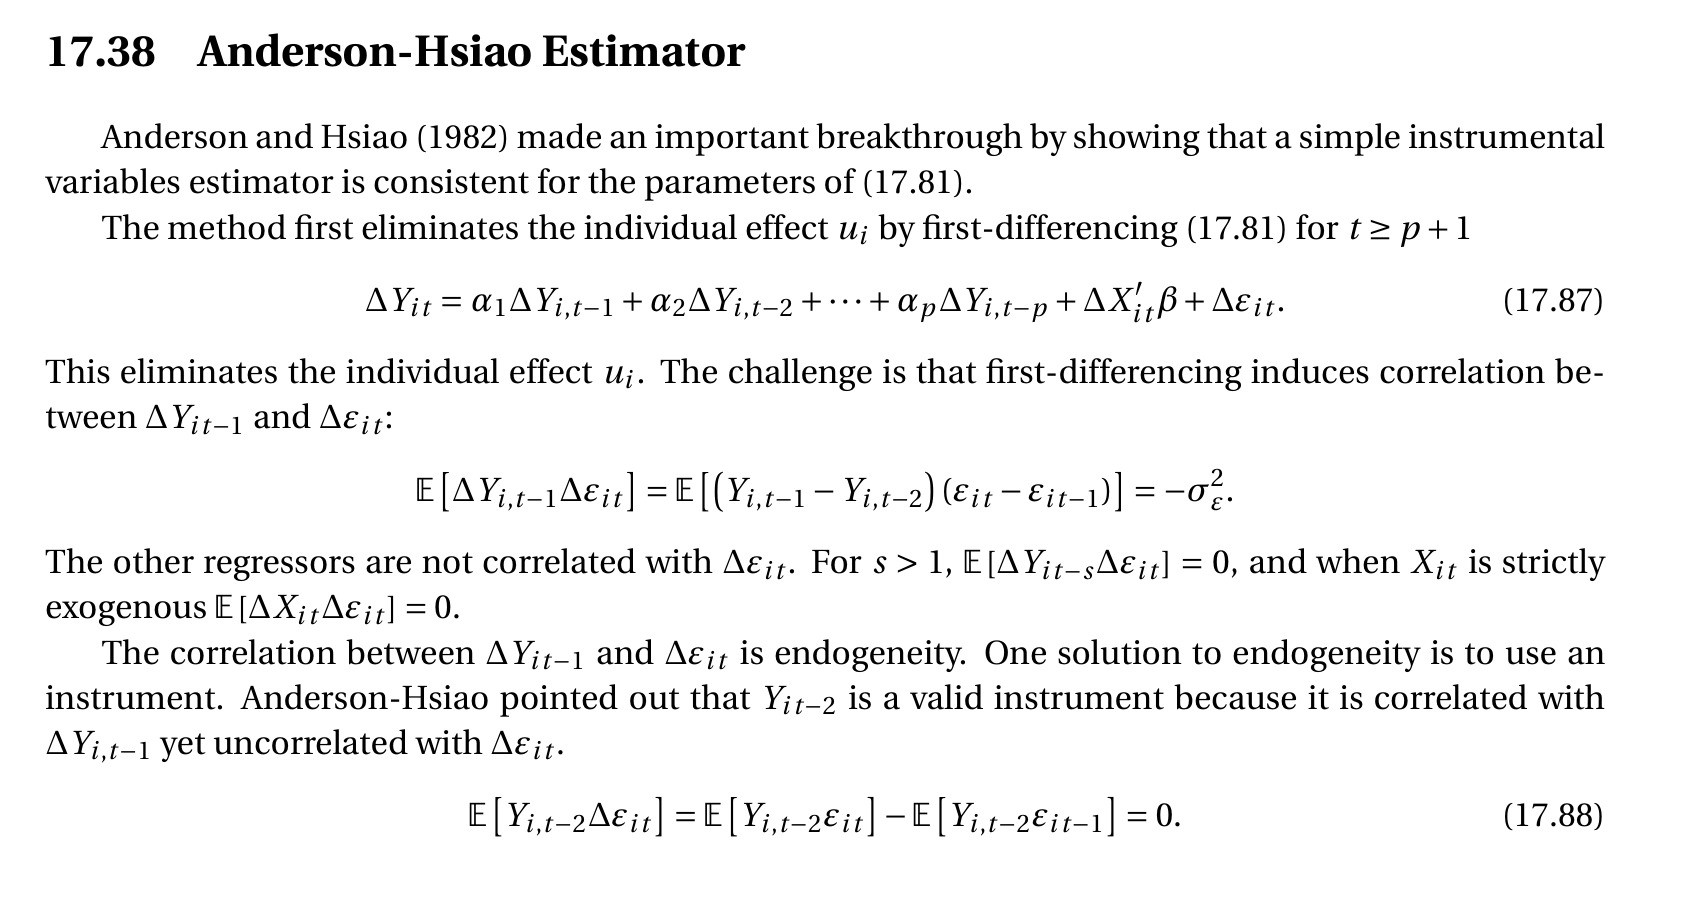
\includegraphics[width=\linewidth]{figures/Anderson-Hsiao-1981.png}
\end{figure}
\begin{figure}
    \centering
    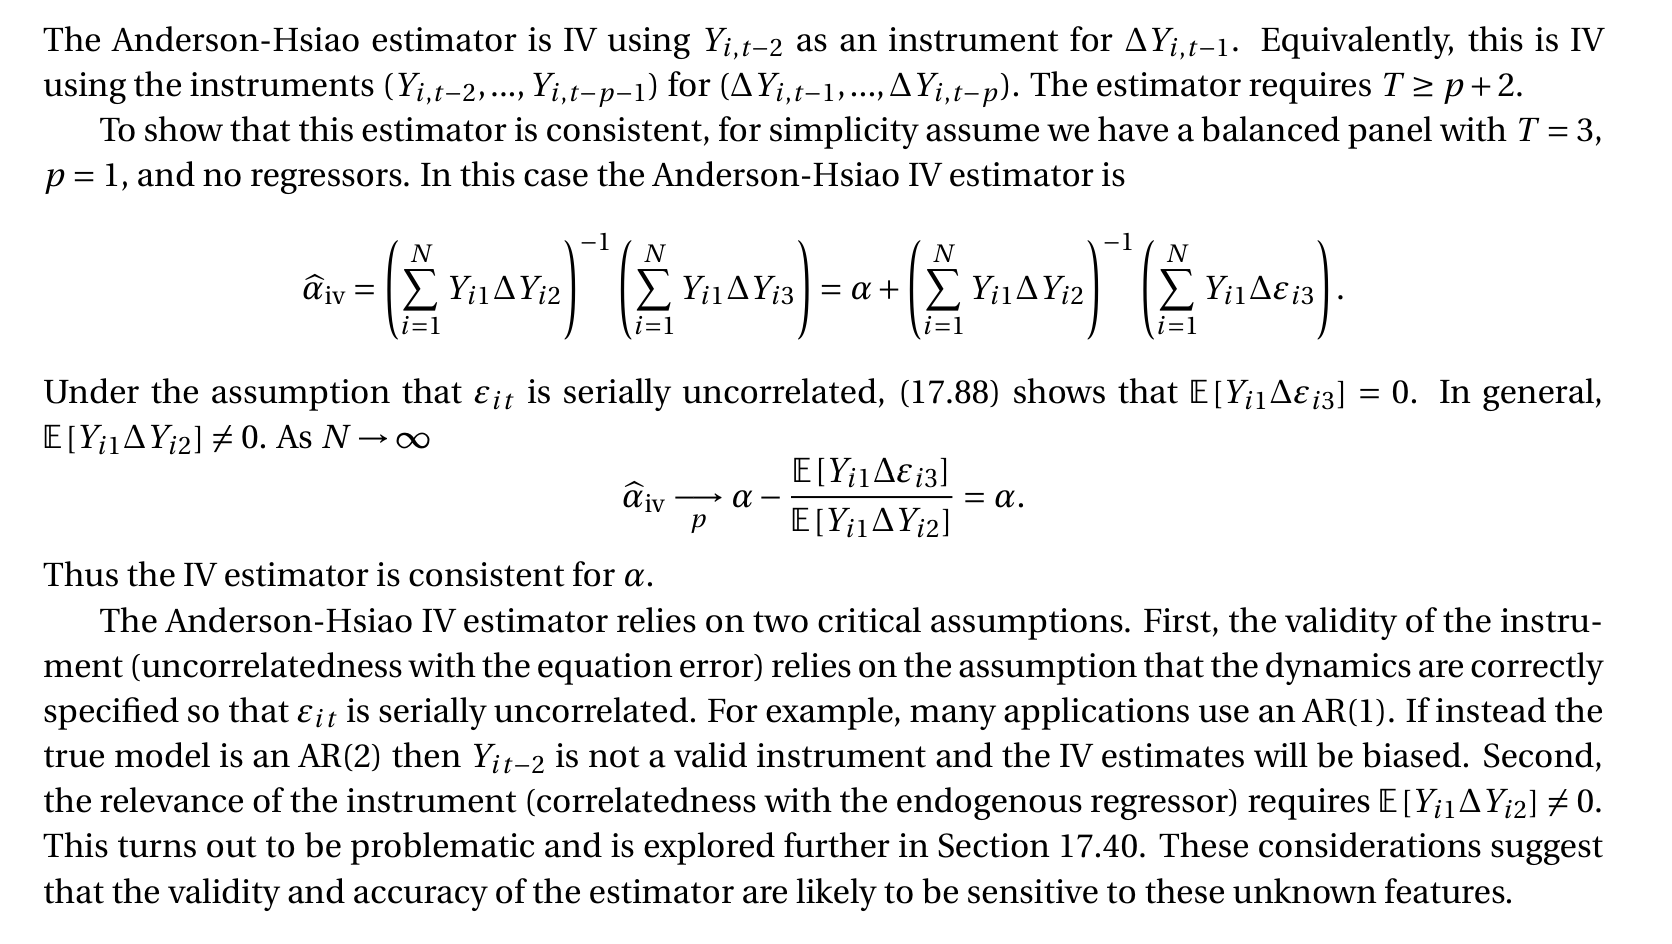
\includegraphics[width=\linewidth]{figures/Anderson-Hsiao-1981-2.png}
    \caption{Anderson and Hsiao(1981)}
\end{figure}

Using similar reasoning, other approaches use sequential exogeneity to circumvent FE meth-
ods altogether rather than to save their consistency. For example, Blundell and Bond (1998)
start from the original specification:
\[y_{it} = x_{it}^{\prime} \beta + \alpha_i + u_{it}, \]
where correlation between $\alpha_{i}$ an $x_{it}$ is suspected to be due to $y_{i,t-1}$, contained in $x_{it}.$

\begin{definition}[Blundell and Bond(1998)]
    \

    \begin{align*}
        y_{it} &= \alpha _i + \beta_1 y_{i,t-1} + u_{it} \\
        &= \beta_1 y_{i,t-1} + (u_{it} + \alpha_i) 
    \end{align*}
    Use $\Delta y_{i,t-1}$ as the IV for $y_{i,t-1}$
\end{definition}

\chapter{Time Series}
\section{Univariate Time Series}

We have a sample $\{w_i\}_{i=1}^n$, with $w_i = (y_i, x_i^{\prime})^{\prime}$, 

$\{w_{it}\}_{i=1:n, t=1:T}$.

Now, we look at $\{w_t\}_{i=1}^T$, usually written as $y_t$, is univariate time series data.

In the cross-sectional context, we average over $i$ to get 
\[\mathbb{E}[u_i] = \int u_i f_u(u_i) d u_i.\]

Under tiem series data, we also think $y_t$ as a RV. without i.i.d. assumption,
we generallt have $T$ realizations of different and mutually dependent variables.

\begin{gather*}
    \mathbb{E}[y_t] = \int y_t f_{y_t}(y_t) d y_t = \mu_t, \\
    \mathbb{V}[y_t] = \mathbb{E}\Bigl[(y_t - \mu_t)^2 \Bigr] = \gamma_{0,t}, \\
    \operatorname{Cov}(y_t, y_{t-h}) = \mathbb{E}\Bigl[ (y_t - \mu_t)(y_{t-h} - \mu_{t-h}  ) \Bigr] = \gamma_{h,t}.
\end{gather*}

\begin{definition}[Weak Stationarity]\label{def:weak-stationarity}
    \

    $y_t$ is a weakly stationary process if
    \begin{enumerate}
        \item $\mu_t = \mu$ for all $t$,
        \item $\gamma_{h,t} = \gamma_h$ for all $t$.
    \end{enumerate}
    autocovariance function (ACF): $\{\gamma_0, \gamma_1, \cdots\}$
    autocorrelation function: $\{\rho_0, \rho_1, \cdots \}$, where $\rho_h = \frac{\gamma_h}{\gamma_0}$.
\end{definition}


% \chapter{Least Squares Estimation of the Linear Regression Model}
% \section{Finite Sample Properties}

\[ y_i = x'_i \beta + u \]
\[ Y = X \beta + U \]
where
\begin{equation*}
  Y = \begin{bmatrix}
    y_1\\
    \vdots\\
    y_n
  \end{bmatrix}_{n \times 1}, \quad
  X = \begin{bmatrix}
    x'_1\\
    \vdots\\
    x'_n
  \end{bmatrix}_{n \times k}, \quad
  U = \begin{bmatrix}
    u_1\\
    \vdots\\
    u_n
  \end{bmatrix}_{n \times 1}
\end{equation*}

\begin{assumption}\label{Assumption 1}
  (Independent Sampling). Observations $z_i = \{ y_t, x_i \}_{i = 1}^n$ are independent across $i$.
\end{assumption}

\begin{assumption}\label{Assumption 2}
  (Full rank). The matrix $X'X = \sum x_i x'_i$ is of full rank.
\end{assumption}

\begin{assumption}\label{Assumption 3}
  (Conditional Independence). $\mathbb{E}[u_i | x_i] = 0$.

  $\mathbb{E}[y_i] = \mathbb{E}[x'_i \beta + u_i | x_i] = \mathbb{E}[x'_i \beta | x_i] + \mathbb{E}[u_i | x_i] = x'_i \beta$
\end{assumption}

\begin{assumption}\label{Assumption 4}  
  (Homoskedasticity). $\mathbb{V}[u_i | x_i] = \sigma^2$ for all $i$.

  $\mathbb{V}[y_i] = \mathbb{V}[x'_i \beta + u_i | x_i] = \sigma^2$
\end{assumption}

The OLS estimator:
\[ \hat{\beta}_{\text{OLS}} = \arg\min_{\beta \in \mathbb{R}^k} 
   \sum u_i^2 = \arg\min_{\beta \in \mathbb{R}^k} \sum_{i = 1}^n
   (y_i - x'_i \beta)^2 = \arg\min_{\beta \in \mathbb{R}^k} (Y - X
   \beta)'(Y - X \beta) \]
   
\begin{align*}
  \frac{\partial (Y - X \beta)'(Y - X \beta)}{\partial \beta} &= X'(Y - X
  \beta) = 0\\
  &\Rightarrow X'Y - X'X\beta = 0\\
  &\Rightarrow (X'X)^{-1}X'Y = \hat{\beta}
\end{align*}

\[ \hat{Y} = X\hat{\beta} = X(X'X)^{-1}X'Y = P_X Y \]
where $P_X = X(X'X)^{-1}X'$ is the projection matrix.
\[ y = x\hat{\beta} + \hat{u} \rightarrow y = \hat{y} + \hat{u} \]
thus,
\[ \hat{U} = Y - \hat{Y} = Y - P_X Y = (I - P_X)Y = M_X Y \]
where $M_X$ is another projection matrix.
\[ Y = P_X Y + M_X Y = (P_X + M_X)Y. \]

In another sense:
\[\hat{U} = Y - \hat{Y} = X\beta + U - X(X^{\prime} X)^{-1}X^{\prime}(X \beta +U) = (I_n - X(X^{\prime} X)^{-1}X^{\prime})U = (I_n - P_X)U = M_{X} U.\]

$P_X$ and $M_X$ are idempotent: $P_X = P'_X$ and $P_X P_X = P_X$, and are orthogonal to each other: $P_X M_X = M_X P_X = 0$.

The total sum of squares (SST) is given by:
\[ \sum_{i = 1}^n y_i^2 = Y'Y \]
It measures the variability in $y_i$ across observations $i$.

We can decompose it into the explained sum of squares (SSE) and the residual sum of squares (SSR)
\begin{align*}
  \text{SST} = Y'Y &= (P_X Y + M_X Y)'(P_X Y + M_X Y)\\
  &= Y'P_X P_X Y + Y'P_X M_X Y + Y'M_X P_X Y + Y'M_X M_X Y \\
  &= Y'P_X P_X Y + Y'M_X M_X Y\\
  &= \hat{Y}'\hat{Y} + \hat{U}'\hat{U}\\
  &= \text{SSE} + \text{SSR}
\end{align*}

Based on that, we get the $R^2$-statistic as a measure of how well $X$ accounts for the variation in $Y$ in the linear regression model:
\[ R^2 = \frac{\hat{Y}'\hat{Y}}{Y'Y} = 1 - \frac{\hat{U}'\hat{U}}{Y'Y}
   \in [0, 1] \left(\frac{\text{SSE}}{\text{SST}} = 1 - \frac{\text{SSR}}{\text{SST}}\right) \]

Look at \textbf{Assumption \ref{Assumption 3}} again, it always gives product have intercept $x_{i1} = 1$.
\begin{align*}
  \mathbb{E}[\hat{\beta} | X] &= \mathbb{E}[(X'X)^{-1}X'Y | X]\\
  &= \mathbb{E}[(X'X)^{-1}X'(X\beta + U) | X]\\
  &= \mathbb{E}[\beta | X] + \mathbb{E}[(X'X)^{-1}X'U | X]\\
  &= \beta + (X'X)^{-1}X'\mathbb{E}[U | X]\\
  &= \beta\\
  \Rightarrow \mathbb{E}[\hat{\beta}] &= \mathbb{E}[\mathbb{E}[\hat{\beta} | X]] = \beta
\end{align*}

For \textbf{Assumption \ref{Assumption 4}}, the conditional variance of $\hat{\beta}_{OLS} $ is given by:
\begin{align*}
  \mathbb{V}[\hat{\beta} | X] &= \mathbb{E}[(\hat{\beta} - \beta)(\hat{\beta} - \beta)' | X]\\
  &= \mathbb{E}[((X'X)^{-1}X'U)((X'X)^{-1}X'U)' | X] \\
  &= \mathbb{E}[(X'X)^{-1}X'UU'X(X'X)^{-1} | X]\\
  &= (X'X)^{-1}X'\mathbb{E}[UU' | X]X(X'X)^{-1}\\
  &= (X'X)^{-1}X'\sigma^2X(X'X)^{-1}\\
  &= \sigma^2(X'X)^{-1}
\end{align*}

\begin{note}
  \begin{eqnarray*}
    UU^{\prime} &=& \begin{bmatrix}
      u_1\\
      \vdots\\
      u_n 
    \end{bmatrix} \begin{bmatrix}
      u_1 & \cdots & u_n
    \end{bmatrix} = \begin{bmatrix}
      u_1^2 & u_1 u_2 & \cdots & u_1 u_n\\
      u_2 u_1 & u_2^2 & \cdots & u_2 u_n\\
      \vdots & \vdots & \ddots & \vdots\\
      u_n u_1 & u_n u_2 & \cdots & u_n^2
    \end{bmatrix}\\
    \mathbb{E}[UU^{\prime} | X] &=& \begin{bmatrix}
      \mathbb{E}[u_1^2 | X] & \mathbb{E}[u_1 u_2 | X] & \cdots & \mathbb{E}[u_1 u_n | X]\\
      \mathbb{E}[u_2 u_1 | X] & \mathbb{E}[u_2^2 | X] & \cdots & \mathbb{E}[u_2 u_n | X]\\
      \vdots & \vdots & \ddots & \vdots\\
      \mathbb{E}[u_n u_1 | X] & \mathbb{E}[u_n u_2 | X] & \cdots & \mathbb{E}[u_n^2 | X]
    \end{bmatrix}
  \end{eqnarray*}
  By \textbf{Assumption \ref{Assumption 3}} and \textbf{Assumption \ref{Assumption 4}}, we have:
  $\mathbb{E}[u_i| X] = 0$ and $\mathbb{E}[u_i^2 | X] = \sigma^2$. Furthermore, $\mathbb{E}[u_i u_j | X] = 0$ for $i \neq j$.
  \begin{eqnarray*}
    \mathbb{E}[UU^{\prime} | X] &=& \sigma^{2} I_{n} 
  \end{eqnarray*}
\end{note}

By LIE again, the unconditional variance of $\hat{\beta}_{OLS}$ is given by:
\begin{align*}
  \mathbb{V}[\hat{\beta}] &= \mathbb{E}[(\hat{\beta} - \beta)(\hat{\beta} - \beta)']\\
  &= \mathbb{E}[\mathbb{E}[(\hat{\beta} - \beta)(\hat{\beta} - \beta)' | X]]\\
  &= \mathbb{E}[\mathbb{V}[\hat{\beta} | X]]\\
  &= \mathbb{E}[\sigma^2(X'X)^{-1}]\\
  &= \sigma^2\mathbb{E}[(X'X)^{-1}]
\end{align*}

\begin{theorem}[Gauss-Markov Theorem]\label{Gauss-Markov Theorem}
  \

  If \textbf{Assumption \ref{Assumption 1}} to \textbf{Assumption \ref{Assumption 4}} hold, then the OLS estimator $\hat{\beta}_{OLS}$ is the best linear unbiased estimator (\textbf{\textcolor{blue}{BLUE}}) of $\beta$.
  \begin{note}
  \
  
    \begin{itemize}
      \item \textbf{Best} means that the OLS estimator has the smallest variance among all linear unbiased estimators. $\mathbb{V}[\hat{\beta}_{OLS}] \leq \mathbb{V}[\hat{\beta}]$ for all linear unbiased estimators $\hat{\beta}$.
      \item \textbf{Linear} means that the estimator is a linear function of the dependent variable. $\hat{\beta} = c + dY$.
      \item \textbf{Unbiased} means that the expected value of the estimator is equal to the true value of the parameter. $\mathbb{E}[\hat{\beta}] = \beta$.
    \end{itemize}
  \end{note}
\end{theorem}

If, we know $\hat{\beta }$, $\mathbb{E}[\hat{\beta}]$ and $\mathbb{V}[\hat{\beta}]$. To find the unconditional expectation of $\hat{\beta}_{OLS}$, we could only use asymptotic properties of the OLS estimator. We can show that the OLS estimator is consistent and asymptotically normal.

\begin{align*}
  \hat{\beta }_{OLS} &= (X'X)^{-1}X'Y\\
  &= (X'X)^{-1}X'(X\beta + U)\\
  &= \beta + (X'X)^{-1}X'U\\
  &= \beta + \left(\sum x_i x'_i\right)^{-1} \left(\sum x_i u_i \right)\\
  &= \beta + \left(\frac{1}{n}\sum x_i x'_i\right)^{-1} \frac{1}{n}\left(\sum x_i u_i \right)\\
  &\overset{p}{\rightarrow} \beta + \mathbb{E}[x_i x'_i]^{-1} \mathbb{E}[x_i u_i]
\end{align*}

\begin{note}
  By WLLN, we know that $\frac{1}{n}\sum{z_i} \overset{p}{\rightarrow} \mathbb{E}[z_i]$.
  So, $\frac{1}{n}\sum x_i u_i \overset{p}{\rightarrow} \mathbb{E}[x_i u_i] = Q$, and $\left[\frac{1}{n}\sum{x_i x^{\prime} _i}\right]^{-1} \overset{p}{\rightarrow} \left\{\mathbb{E}[x_i x^{\prime} _i]\right\}^{-1} \overset{p}{\rightarrow} \mathbb{E}[x_i x^{\prime} _i]^{-1} = Q^{-1} .$
\end{note}

So, we have:
\begin{align*}
  \hat{\beta}_{OLS} - \beta &\overset{p}{\rightarrow} \mathbb{E}[x_i x'_i]^{-1} \mathbb{E}[x_i u_i]\\
  &= \mathbb{E}[x_i x'_i]^{-1} \mathbb{E}[\mathbb{E}[x_i u_i | x_i]]\\
  &= \mathbb{E}[x_i x'_i]^{-1} \mathbb{E}[x_i \mathbb{E}[u_i | x_i]]\\
  &= \mathbb{E}[x_i x'_i]^{-1} \mathbb{E}[x_i \cdot 0]\\
  &= 0
\end{align*}

\begin{note}
  By the Central Limit Theorem, 
  we know that:
  \begin{align*}
    \sqrt{n}(\hat{\beta}_{OLS} - \beta) &= (X^{\prime} X)^{-1}X^{\prime} U \\
    &= \underset{\mathbb{E}[x_i x^{\prime} _i]^{-1}}{\underbrace{\left(\frac{1}{n}\sum x_i x'_i\right)^{-1}}} \sqrt{n} \underset{\overset{d}{\rightarrow} \mathcal{N}(0, \mathbb{V}[x_i u_i])}{\underbrace{\frac{1}{n}\sum x_i u_i}} \\
    & \overset{p}{\rightarrow} \mathbb{E}[x_i x^{\prime} _i]^{-1} \mathcal{N}(0, \mathbb{V}[x_i u_i])
  \end{align*}
\end{note}

Thus, we have:
\begin{align*}
  \sqrt{n}(\hat{\beta}_{OLS} - \beta) &\overset{d}{\rightarrow} \mathcal{N} (0, \mathbb{E}[x_i x^{\prime} _i]^{-1}\mathbb{V}[x_i u_i] \mathbb{E}[x_i x^{\prime} _i]^{-1^{\prime} } )\\
  \mathbb{V}[x_i u_i] &= \mathcal{N}(0, \mathbb{E}\left[(x_i u_i - \mathbb{E}[x_i u_i])(x_i u_i - \mathbb{E}[x_i u_i])^{\prime} \right]) \\
  &= \mathcal{N} (0, \mathbb{E}[x_i u_i u_i^{\prime} x_i] - \mathbb{E}[x_i u_i] \mathbb{E}[x_i u_i]^{\prime})\\
  &= \mathcal{N} (0, \mathbb{E}[x_i u_i u_i^{\prime} x_i^{\prime} ])\\
  &= \mathcal{N} (0, \mathbb{E}[\mathbb{E}[u_i^2 | x_i] x_i x_i^{\prime}])\\
  &= \mathcal{N} (0, \mathbb{E}[\sigma^2 x_i x_i^{\prime}])\\
  &= \sigma^2 \mathbb{E}[x_i x_i^{\prime}]\\
  &= \sigma ^2 Q \\
  \Rightarrow \sqrt{n}(\hat{\beta}_{OLS} - \beta) &\overset{d}{\rightarrow} \mathcal{N} (0, \mathbb{E}[x_i x^{\prime} _i]^{-1} \sigma^2 \mathbb{E}[x_i x_i^{\prime}] \mathbb{E}[x_i x^{\prime} _i]^{-1} ) = \mathcal{N} (0, \sigma^2 Q^{-1})
\end{align*}

Then,  we could say that:
\begin{itemize}
  \item For finite $n$, $\sqrt{n}(\hat{\beta}_{OLS} - \beta) \overset{approx}{\sim} \mathcal{N} (0, \sigma ^2 Q^{-1});$
  \item $\hat{\beta } \overset{approx}{\sim} \mathcal{N} (\beta , \frac{\sigma^2}{n} Q^{-1})$;
  \item Replace unknown $\sigma^2$ and $Q^{-1}$ by $\hat{\sigma}^2$ and $\hat{Q}^{-1}$ to get the t-distribution.
  We would have: \[\hat{\beta } \overset{approx}{\sim} \mathcal{N} \left(\beta , \frac{\hat{\sigma}^2}{n} \hat{Q}^{-1}\right).\]
\end{itemize}

\section{Hypothesis Testing}
As $\hat{\beta } \overset{approx}{\sim} \mathcal{N} \left(\beta , \frac{\hat{\sigma}^2}{n} \hat{Q}^{-1}\right)$,
we know that:
\[\hat{\beta}_j \overset{approx}{\sim} \mathcal{N}(\beta_{j}, \frac{\hat{\sigma}^2}{n}[\hat{Q}^{-1}]_{jj})\] for a single parameter $\beta_j \in \beta$
where $[\hat{Q}^{-1}]_{jj}$ is the $j$-th diagonal element of $\hat{Q}^{-1}$.

This enables us to test a point hypothesis $\mathcal{H}_{0}: \beta_j = \beta_{j, 0}$ against the alternative $\mathcal{H}_{1}: \beta_j \neq \beta_{j, 0}$ using the t-test:
\[\varphi_t(x) =\mathbf{1}\left\{T_x < c\right\}, \text{with } T_t = \left| \frac{\hat{\beta}_{j,0} - \beta_j}{\hat{\sigma}_{\beta_{j,0}}} \right|,\]
where $\hat{\sigma}_{\beta_{j,0}} = \sqrt{\frac{\hat{\sigma}^2}{n}\hat{Q}_{jj}^{-1}}.$

Because the distribution of $\hat{\beta}_j$ is not exact, but only asymptotically valid, so too does the
resulting test-statistic only asymptotically converge to a standard Normal distribution:
\[t = \frac{\hat{\beta}_j - \beta_{j, 0}}{\sqrt{\frac{\hat{\sigma}^2}{n}[\hat{Q}^{-1}]_{jj}}} \overset{d}{\rightarrow} \mathcal{N}(0, 1)\]

\begin{align*}
  \hat{\beta _j} &\overset{approx}{\sim} \mathcal{N} \left(\beta _j , \underset{V_j}{\underbrace{\frac{\sigma^2}{n}\left(\frac{1}{n} \sum{x_i x_i^{\prime} }\right)^{-1}_{jj}}} \right)\\
  t &= \frac{\hat{\beta _j} - \beta _j}{\sqrt{V_j}} \overset{approx}{\sim} \mathcal{N} (0, 1)\\
\end{align*}

\begin{definition}[Wald Test]\label{Wald Test}
  \ 

  The asymptotic distribution of the Wald-test-statistic, $T_W$,
  follows from asymptotic Normality of $\hat{\beta}$, 
  the Delta Method and the fact that $(X-\mu)^\prime\Sigma^{-1}(X-$ $\mu)\sim\chi_{dim(X)}^2$ for $X\sim N(\mu,\Sigma).$

  Using $\sqrt{n}(\hat{\beta}-\beta_{0})\stackrel{d}{\rightarrow}N(0,V)$ and the Delta method, we get
  $$\sqrt{n}\left(g(\hat{\beta})-g(\beta_0)\right)\overset{d}{\to}G\cdot N(0,V)=N(0,GVG')\:,\quad\mathrm{with}\quad G=\left.\frac{\partial g(\beta)}{\partial\beta}\right|_{\beta=\beta_0}\:.$$
  Therefore,
  $$\sqrt{n}\left(g(\hat{\beta})-g(\beta_0)\right)'[GVG']^{-1}\sqrt{n}\left(g(\hat{\beta})-g(\beta_0)\right)\stackrel{d}{\to}\chi_m^2\:.$$

  Under $\mathcal{H}_0: g(\beta_0)=0.$ Also, because we do not know $\beta_0$, we replace $G$ with $G(\hat{\beta})$, as $\hat{\beta}$ is our
  estimator of $\beta_0.$
\end{definition}

More general hypotheses  $\mathcal{H}_{0}: g(\beta)=0 $ vs.  $\mathcal{H}_{1}: g(\beta) \neq 0$  for some function  $g: \mathbb{R}^{k} \rightarrow \mathbb{R}^{m}$  (i.e. $ m \leq k $ restrictions) can be tested using the Wald test. It uses the following statistic:

$$T_{W}=n g\left(\hat{\beta}_{O L S}\right)^{\prime}\left[G\left(\hat{\beta}_{O L S}\right) \hat{V} G\left(\hat{\beta}_{O L S}\right)^{\prime}\right]^{-1} g\left(\hat{\beta}_{O L S}\right) \xrightarrow{d} \chi_{m}^{2},$$

where $\hat{V}=\hat{\sigma}^{2} \hat{Q}^{-1}$ and where  $G\left(\hat{\beta}_{O L S}\right)=\partial g(\beta) /\left.\partial \beta\right|_{\beta=\hat{\beta}_{O L S}}$  is the $m \times k$ matrix of derivatives of $g$ with respect to $\beta$  evaluated at  $\hat{\beta}_{OLS}$. 
The short derivation in the Appendix illustrates that the Wald test-statistic is based on the idea that if $\mathcal{H}_{0}$  is true, then the difference between  $g\left(\hat{\beta}_{O L S}\right)$ and $g(\beta)=0$ should be small. Suppose we are interested in testing  $\mathcal{H}_{0}:\left\{\beta_{2}+\beta_{3}=5, \beta_{4}=0\right\}$ under a five-dimensional vector $\beta$. 
Then we would take
\[
g(\beta)=\left[\begin{array}{lllll}
0 & 1 & 1 & 0 & 0 \\
0 & 0 & 0 & 1 & 0
\end{array}\right] \beta-\left[\begin{array}{l}
5 \\
0
\end{array}\right], \quad \text { with } \quad G(\beta)=\left[\begin{array}{lllll}
0 & 1 & 1 & 0 & 0 \\
0 & 0 & 0 & 1 & 0
\end{array}\right]
\]

If $g(\beta)=0$ is s.t. it tests only $\beta_{j}=\beta_{j, 0}$ for a single $\beta_{j}$ , then the Wald test is equivalent to the t-test:  $\varphi_{W}=\varphi_{t}$.

\begin{theorem}[Delta Method]
  \

  $X \overset{d}{\rightarrow}\mathcal{N} (\mu, \sigma^2)$, and $g: \mathbb{R}^k \rightarrow \mathbb{R}^q$ is a differentiable function. 
  Then, $g(X) \overset{d}{\rightarrow} \mathcal{N} (g(\mu), \sigma^2(g'(\mu))^2)$.

  Let $\beta \in \mathbb{R}^k$ and $g: \mathbb{R}^k \rightarrow \mathbb{R}^q$ be a differentiable function.
  If $\sqrt{n}(\hat{\beta} - \beta) \overset{d}{\rightarrow} \xi$, then
  \[ 
  \sqrt{n}(g(\hat{\beta}) - g(\beta)) \overset{d}{\rightarrow} G^{\prime} \xi,
  \]
  where $G = G(\beta) = \frac{\partial}{\partial \beta}g(\beta)^{\prime}.$

  In particular, if $\xi \sim \mathcal{N}(0, V)$, then
  \[\sqrt{n}(g(\hat{\beta}) - g(\beta)) \overset{d}{\rightarrow} \mathcal{N}(0, G V G^{\prime}).\]

  By previous results, if we have $V = \sigma^2 Q^{-1}$, then
  \[ 
    \sqrt{n}(g(\hat{\beta}) - g(\beta)) \overset{d}{\rightarrow} \mathcal{N} (0, G \sigma^2 Q^{-1} G^{\prime})
  \]
  where $G(u) = \frac{\partial}{\partial u}g(u)^{\prime} $ and $G = G(\beta )$.
\end{theorem}

\section{Violations of Ideal Conditions}

First of all, note that while unbiasedness requires the conditional independence assumption
3 to hold, both consistency and asymptotic Normality go through even under the weaker
exogeneity assumption $\mathbb{E}[u_i x_i] = 0.$\footnote{This is because it's implied by the conditional independence assumption.}

\subsection{Singular $X^{\prime} X$}
If $X^{\prime} X$ is not of full rank, then the OLS estimator is not even defined. There are two reasons
that lead to this case.

\subsection{Heteroskedasticity}
Suppose we replace the Assumption \ref{Assumption 4} with the weaker assumption that $\mathbb{V}[u_i | x_i] = \sigma^2_i$ for all $i$.
Then, the OLS estimator is still unbiased, but the variance of the OLS estimator is now given by:
\begin{align*}
  \mathbb{V}[x_i u_i] &= \mathbb{E}[\left(x_i u_i - \mathbb{E}[x_i u_i]\right) \left(x_i u_i - \mathbb{E}[x_i u_i]\right)^{\prime}]\\
  &= \mathbb{E}[x_i u_i u_i^{\prime}  x_i^{\prime}] - \mathbb{E}[x_i u_i] \mathbb{E}[x_i u_i]^{\prime}\\
  &= \mathbb{E}[\mathbb{E}[u_i^2 | x_i] x_i x_i^{\prime}]\\
  &= \mathbb{E}[x_i x_i^{\prime} u_i^2] \\
  &= \mathbb{E}[x_i x_i^{\prime} \sigma^2_i] \\
  \Rightarrow \sqrt{n}(\hat{\beta}_{OLS} - \beta) &\overset{d}{\rightarrow} \mathcal{N} (0, Q^{-1} \mathbb{E}[x_i x_i^{\prime} u_i^2] Q^{-1})  
\end{align*}

The asymptotic variance can again be estimated by replacing $\mathbb{E}[x_i x_i^{\prime} u_i^2]$ with its sample analogue:
as a consistent estimator: $\frac{1}{n}\sum_{i=1}^{n} x_i x_i^{\prime} \hat{u}_i^2.$

Note that if the variances $\{\sigma_i^2\}_{i=1}^n$ were known, we could transform the heteroskedastic model
into a homoskedastic one by writing the regression as:
\[ \frac{y_i}{\sigma_i} = \frac{x_i^{\prime} }{\sigma_i} \beta + \frac{u_i}{\sigma_i}. \]

In this model, observations are weighted by the inverses of their standard deviations and, as
a result, less noisy observations are given more weight as they are more informative about
the relation between $X$ and $Y$. Let $\mathbb{V}[U|X] = \Sigma = diag{(\sigma_1^2, \cdots, \sigma_n^2)}.$
We can then write the regression in matrix form as:
$\Sigma^{-\frac{1}{2}}Y = \Sigma^{-\frac{1}{2}}X \beta + \Sigma^{-\frac{1}{2}}U,$
with $\mathbb{V}[\Sigma^{-\frac{1}{2}}U|X] = I.$

The OLS estimator in this weighted regression model is referred to as the Generalized Least Squares (GLS) estimator.
It is given by:
\[ \hat{\beta}_{GLS} = \left(\left(\Sigma^{-\frac{1}{2}}X \right)^{\prime}\left(\Sigma^{-\frac{1}{2}}X \right)\right)\left(\Sigma^{-\frac{1}{2}}X \right)^{\prime} \left(\Sigma^{-\frac{1}{2}}Y \right)  = (X^{\prime} \Sigma^{-1} X)^{-1} X^{\prime} \Sigma^{-1} Y. \]

Under otherwise the same conditions as for OLS, this estimator is unbiased\footnote{$\mathbb{E}\left[\hat{\beta}_{GLS}|X\right] = \mathbb{E}\left[\left(X^{\prime} \Sigma^{-1} X\right)^{-1}(X\beta+U)|X \right] = \beta + \mathbb{E}\left[\left(X^{\prime} \Sigma^{-1} X\right)^{-1}U|X\right]=\beta.$} 
and consistent\footnote{$\hat{\beta}_{GLS} - \beta = (X^{\prime} \Sigma^{-1} X)^{-1}X^{\prime} \Sigma^{-1} U \overset{p}{\rightarrow} \frac{1}{n}\mathbb{E}\left[\frac{x_i x_i^{\prime}}{\sigma_i^2}\right] \frac{1}{n}\mathbb{E}\left[\frac{x_i u_i}{\sigma_i^2}\right] \overset{p}{\rightarrow} 0.$}.
and has variance: 
\[
\mathbb{V}[\hat{\beta}_{GLS}] = \mathbb{E}\left[(X^{\prime} \Sigma^{-1} X)^{-1} X^{\prime} \Sigma^{-1} U U^{\prime} \Sigma^{-1} X (X^{\prime} \Sigma^{-1} X)^{-1}\right] = \mathbb{E}\left[(X^{\prime} \Sigma^{-1} X)^{-1}\right].
\]

\subsection{Endogeneity}
\subsubsection{Omitted Variables}
Suppose the true model is given by:
$$y_i=x_i'\beta+z_i'\delta+\varepsilon_i\:,\text{with } \mathbb{E}[x_i\varepsilon_i]=0,$$
i.e. exogeneity holds in this true model, whereas the researcher estimates
$$y_i = x_i^{\prime} \gamma+u_i.$$

Notice that we have written the coefficient as $\gamma$ rather than $\beta$ and the error as $u$ rather than $\varepsilon .$ Goldberger (1991) introduced the catchy labels long regression and short regression to emphasize the distinction.
Typically, $\beta\neq\gamma$,except in special cases. To see this, we calculate
\begin{align*}
  \gamma&=\left(\mathbb{E}\left[XX^{\prime}\right]\right)^{-1}\mathbb{E}\left[XY\right]\\
  &=\left(\mathbb{E}\left[X X^{\prime}\right]\right)^{-1}\mathbb{E}\left[X \left(X^{\prime}\beta + Z^{\prime}\delta+\varepsilon\right)\right]\\
  &=\beta+\left(\mathbb{E}\left[X X^{\prime}\right]\right)^{-1}\mathbb{E}\left[X Z^{\prime}\right]\delta\\
  &=\beta+\Gamma\delta
\end{align*}

where $\Gamma=Q^{-1}Q_{XZ}$ is the coefficient matrix from a projection of $Z$ on $X$.

Observe that $\gamma=\beta+\Gamma\delta\neq\beta$ unless $\Gamma=0$ or $\delta=0.$ Thus the short and long regressions have different coefficients. 
They are the same only under one of two conditions. 
First, if the projection of $Z$ on $X$ yields a set of zero coefficients (they are uncorrelated), 
or second, if the coefficient on $Z$ in is zero. 
The difference $\Gamma\delta$ between $\gamma$ and $\beta$ is known as omitted variable bias. 
It is the consequence of omission of a relevant correlated variable.


% \chapter{Likelihood-Based Inference}
% In previous lectures we have discussed the least squares estimation of the linear regression model. In this lecture we will discuss the likelihood-based inference.
\begin{table}[h!]
    \centering
    \begin{tabular}{c|c|c}
        \hline
         & ch2 & ch3(LRM) \\
        \hline
        LS & $\mathbb{E}[y_i|\theta]$ & $\mathbb{E}[y_i|x_i, \beta]$ \\
        ML & $p(y_i | \theta )$ & $p(y_i|x_i, \beta )$ \\
        \hline
    \end{tabular}
\end{table}

\section{ML for LRM}
\[y_i = x^{\prime} _i \beta + u_i\]
For LS, we assume $\mathbb{E}[u_i|x_i] = 0$, which gives $\mathbb{E}[y_i|x_i] = x^{\prime} _i \beta.$
For ML, we assume $u_i \sim N(0, \sigma^2)$, which gives $y_i|x_i \sim N(x^{\prime} _i \beta, \sigma^2).$
\[
p(y_i|x_i) = (2\pi \sigma^2)^{-\frac{1}{2}} \exp\left\{ -\frac{1}{2 \sigma ^2} (y_i - x^{\prime} _i \beta )^2\right\}
\]
We use $\theta $ to represent parameters $(\beta, \sigma^2).$
\begin{align*}
    \Rightarrow \mathcal{L}(\theta |y_i, x) &= p(y | x_i, \theta ) \\
    &= \prod_{i=1}^{n}p(y_i|x_i,\theta )\\
    &= \prod_{i=1}^{n} (2\pi \sigma^2)^{-\frac{1}{2}} \exp\left\{ -\frac{1}{2 \sigma ^2} (y_i - x^{\prime} _i \beta )^2\right\}\\
    &= (2\pi \sigma^2)^{-\frac{n}{2}} \exp\left\{ -\frac{1}{2 \sigma ^2} \sum_{i=1}^{n}(y_i - x^{\prime} _i \beta )^2\right\}
\end{align*}

Then, we can get the log-likelihood function:
\begin{align*}
    \ell(\theta |y_i, x) &= \log \mathcal{L}(\theta |y_i, x)\\
    &= -\frac{n}{2} \log (2\pi \sigma^2) - \frac{1}{2 \sigma ^2} (Y - X\beta )^{\prime} (Y - X\beta )\\
    \Rightarrow \hat{\theta }_{ML} &= (\hat{\beta}_{ML}, \hat{\sigma}^2_{ML}) = \arg\max_{\theta=(\beta, \sigma^2) } \ell(\theta |y_i, x)
\end{align*}

Take the first order condition (FOC) of $\beta$ and $\sigma^2$:
\begin{align*}
    \beta: &\frac{1}{\sigma^2}X'(Y - X\beta ) = 0\\
    \Rightarrow\hat{\beta}_{ML} &= (X'X)^{-1}X'Y\\
    \sigma^2:& -\frac{n}{2\sigma^2} + \frac{2}{(2\sigma^2)^2} (Y - X\beta)'(Y - X\beta) = 0\\
    \Rightarrow \hat{\sigma}^2_{ML} &= \frac{1}{n} (Y - X\beta)'(Y - X\beta) = \frac{1}{n} \sum_{i=1}^{n} \hat{u}^2_i = \hat{\sigma}^2_{LS}
\end{align*}

As we know that:
\[\hat{\beta } = (X^{\prime} X)^{-1}X^{\prime} Y = \beta +(X^{\prime} X)^{-1}X^{\prime} U = \beta + \left(\frac{1}{n}\sum x_i x^{\prime} _i \right)^{-1}\sum x_i u_i\]
\[\Rightarrow \hat{\beta }|X \sim \mathcal{N} (\beta , V)\]
where
\begin{align*}
    V &= \mathbb{V}\left[(X^{\prime} X)^{-1}X^{\prime} U |X\right]\\
    &= (X^{\prime} X)^{-1}\mathbb{V}[X^{\prime} U|X](X^{\prime} X)^{-1}\\
    &= (X^{\prime} X)^{-1}X^{\prime} \mathbb{V}[U|X] X(X^{\prime} X)^{-1}\\
    &= (X^{\prime} X)^{-1}X^{\prime} \sigma^2 I X(X^{\prime} X)^{-1}\\
    &= \sigma^2 (X^{\prime} X)^{-1}
\end{align*}

We define the \textbf{Score Function} as:
\begin{definition}[Score Function]
    \begin{align*}
        S(\theta ) &= \frac{\partial \ell(\theta |y_i, x)}{\partial \theta }\\
        &= \begin{bmatrix}
            \frac{\partial \ell(\theta |y_i, x)}{\partial \beta }\\
            \frac{\partial \ell(\theta |y_i, x)}{\partial \sigma^2}
        \end{bmatrix}
    \end{align*}
\end{definition}


As we know that:
\begin{align*}
    \frac{\partial \ell(\theta |y_i, x)}{\partial \beta } &= \frac{1}{\sigma^2}X'(Y - X\beta )\\
    \frac{\partial \ell(\theta |y_i, x)}{\partial \sigma^2} &= -\frac{n}{2\sigma^2} + \frac{1}{2(\sigma^2)^2} (Y - X\beta )'(Y - X\beta )
\end{align*}

We take the Hessians of $\beta$ and $\sigma^2$:
\begin{align*}
    \mathcal{H} (\theta ) &= \frac{\partial^2 \ell(\theta |y_i, x)}{\partial \theta \partial \theta ^{\prime}} = \frac{\partial S(\theta )}{\partial \theta^{\prime}}\\
    &= \begin{bmatrix}
        \frac{\partial^2 \ell(\theta |y_i, x)}{\partial \beta \partial \beta} & \frac{\partial^2 \ell(\theta |y_i, x)}{\partial \beta \partial \sigma^2}\\
        \frac{\partial^2 \ell(\theta |y_i, x)}{\partial \sigma^2 \partial \beta} & \frac{\partial^2 \ell(\theta |y_i, x)}{\partial \sigma^2 \partial \sigma^2}
    \end{bmatrix}\\
    \frac{\partial^2 \ell(\theta |y_i, x)}{\partial \beta \partial \beta } &= -\frac{1}{\sigma^2}X^{\prime} X\\
    \frac{\partial^2 \ell(\theta |y_i, x)}{\partial \sigma^2 \partial \sigma^2} &= \frac{n}{2(\sigma^2)^2} - \frac{1}{(\sigma^2)^3} (Y - X\beta )'(Y - X\beta )\\
    \frac{\partial^2 \ell(\theta |y_i, x)}{\partial \beta \partial \sigma^2} &= \frac{1}{(\sigma^2)^2}X'(Y - X\beta )
\end{align*}

    
Then, we can get the \textbf{Information Matrix} as: 
\begin{definition}[Information Matrix]
    \begin{align*}
        I(\theta ) &= \mathbb{E}[s(\theta )s(\theta )^{\prime}] =  -\mathbb{E}\left[\frac{\partial^2 \ell(\theta |y_i, x)}{\partial \theta \partial \theta ^{\prime}}\right]\\
        &= -\mathbb{E}\left[\begin{bmatrix}
            \frac{\partial^2 \ell(\theta |y_i, x)}{\partial \beta \partial \beta } & \frac{\partial^2 \ell(\theta |y_i, x)}{\partial \beta \partial \sigma^2}\\
            \frac{\partial^2 \ell(\theta |y_i, x)}{\partial \sigma^2 \partial \beta} & \frac{\partial^2 \ell(\theta |y_i, x)}{\partial \sigma^2 \partial \sigma^2}
        \end{bmatrix}\right]
    \end{align*}
\end{definition}

\begin{align*}
    \mathbb{E}[s(\beta )s(\beta )^{\prime} ] &= -\mathbb{E}\left[ \frac{1}{\sigma ^2}X^{\prime}(Y - X\beta)\left[\frac{1}{\sigma^2} X^{\prime} (Y-X\beta) \right]^{\prime} \right]\\
    &= \mathbb{E}\left[\frac{1}{\sigma^4}X^{\prime}U U^{\prime} X\right]\\
    &= \frac{1}{\sigma^4}X^{\prime} \mathbb{E}[U U^{\prime}] X\\
    &= \frac{1}{\sigma^4}X^{\prime} \sigma^2 I X\\
    &= \frac{1}{\sigma^2}X^{\prime}X \\
    &= \mathbb{E}[-\mathcal{H}(\beta )]
\end{align*}

Then, we could have the \textbf{Cramer-Rao Lower Bound}:
\begin{definition}[Cramer-Rao Lower Bound]
    \ 

    Let $\tilde{\theta }$ be an unbiased estimator of $\theta $, then:
    \begin{align*}
        \mathbb{V}[\tilde{\theta }|X] &\geq I^{-1}(\theta )\\
        &= \sigma^2 (X^{\prime}X)^{-1}
    \end{align*}
\end{definition}

Take a model $\ell(\theta |y)$, and
\begin{align*}
    \hat{\theta} &= \argmax_{\theta}\ell(\theta|y) \\
    \bar{\theta} &= \argmax_{\theta, g(\theta)=0} \ell(\theta|y)
\end{align*}

and $\sqrt{n}(\hat{\theta_0} - \theta) \overset{d}{\rightarrow} \mathcal{N}(0, V)$. 
We want to test: $\mathcal{H}_0: g(\theta)=0.$
Previously, we have three tests:
\begin{itemize}
    \item t-test: $t = \frac{\hat{\theta} - \theta_0}{\sqrt{\frac{1}{n}\hat{V}}} \overset{d}{\rightarrow} \mathcal{N}(0, 1)$
    \item Wald Test: $W = n g(\hat{\theta})^{\prime} [G(\hat{\theta})\hat{V}G(\hat{\theta})^{\prime}]^{-1}g(\hat{\theta}) \sim \chi_k^2$
    \item LR Test: $LR = -2(\ell(\hat{\theta}_0) - \ell(\bar{\theta})) \sim \chi_k^2$
    \item LM Test: $LM = S(\bar{\theta})^{\prime}  I(\bar{\theta})^{-1} S(\bar{\theta}) \sim \chi_k^2$
\end{itemize}


% \chapter{Likelihood-Based Inference(2)}
% \section{Binary Choice: Logit Model \& Probit Model}

Suppose $y_i \in \{0, 1\}$, the common approach is still:
\begin{align*}
    y_i &= x^{\prime} _i \beta + u_i\\
    \mathbb{E}[u_i|x_i] &= 0
\end{align*}
But, the linear regression is not attractive, because $\mathbb{E}[y_i|x_i] = \mathbb{P}[y_i=1|x_i]$ 
is bounded between 0 and 1, while the linear regression is unbounded.

We define a new regression model:
\begin{align*}
    y_i^* = x^{\prime} _i \beta + u_i \\
    u_i|x_i \sim \mathcal{N}(0, 1)
\end{align*}
and assume we have: $y_i = \mathbf{1}\{y_i^* \geq 0\}.$
If utility is positive $y_i=1$, if it is negative, $y_i=0$.

Then, we have the probability of $y_i=1$ as:
\[ 
\mathbb{P}[y_i=1]=\mathbb{P}[x_i^{\prime} \beta + u_i \geq 0] = \mathbb{P}[u_i \geq -x_i^{\prime} \beta] = 1 - \Phi(-x_i^{\prime} \beta)= \Phi(x_i^{\prime} \beta)
\]
and $\mathbb{P}[y_i=0] = 1 - \Phi(x_i^{\prime} \beta)=\Phi(-x^{\prime}_i \beta )$,
where $\Phi $ is the CDF of a standard normal RV.

Hence, $y_i$ had the PDF:
\[
p(y_i|x_i, \beta ) = \left\{\begin{matrix}
   \Phi (x_i^{\prime} \beta ) & y_i = 1\\
   \Phi (-x_i^{\prime} \beta) & y_i = 0
  \end{matrix}\right. = \Phi(x_i^{\prime} \beta )^{y_i} \Phi(-x_i^{\prime} \beta )^{1-y_i}
\]
which is the Bernoulli distribution with probability of success $\Phi(x_i^{\prime} \beta )$.

This leads to our likelihood function:
\begin{align*}
    \mathcal{L}(\beta |Y, X) &= \prod_{i=1}^{n} p(y_i|x_i, \beta )\\
    &= \prod_{i=1}^{n} \Phi(x_i^{\prime} \beta )^{y_i} \Phi(-x_i^{\prime} \beta )^{1-y_i}
\end{align*}
    
Then, we can get the log-likelihood function:
\begin{align*}
    \ell(\beta |Y, X) &= \log \mathcal{L}(\beta | Y, X)\\
    &= \sum_{i=1}^{n} \left\{y_i \log \Phi(x_i^{\prime} \beta ) + (1-y_i) \log \Phi(-x_i^{\prime} \beta )\right\}
\end{align*}
where we have the estimator defines as: $\hat{\beta} = \arg \max_{\beta} \ell(\beta|Y,X).$

Then, we can have:
\[ 
\hat{y_i} = \mathbb{E}[y_i|x_i^{\prime}, \beta ] = \Phi(x_i^{\prime} \hat{\beta}) \Rightarrow R^2 = \frac{\hat{Y}^{\prime} \hat{Y}}{Y^{\prime} Y}.
\]

The partial effect of $X$ on $Y$ is:
\begin{align*}
    \delta &= \mathbb{E}[y_i|x_i=x_2, \beta] - \mathbb{E}[y_i|x_i=x_1, \beta] \\
    &= \Phi(x_2^{\prime} \beta ) - \Phi(x_1^{\prime} \beta )\\
\end{align*}
approximately,
\[
\frac{\partial \mathbb{E}[y_i|x_i \beta]}{\partial x_i} = \frac{\partial \Phi(x_i^{\prime} \beta)}{\partial x_i} = \phi(x_i^{\prime} \beta) \beta.
\]
which is: 
\[
\Delta \mathbb{E}[y_i|x_i \beta] = \phi(x_i^{\prime} \beta ) \beta \Delta x_i.
\]

Since $\Phi(\cdot)$ is a strictly increasing function, 
the sign of $\beta_j$ reveals the sign of the partial effect of $x_{j}$,
but the size of $\beta_{j}$ is not interpretable. 
Only the relative sizes of two coefficients $\beta_k$ and $\beta_{l}$ 
have (qualitative) meaning. Nevertheless, 
we can test for the partial effect of $x_j$ being zero 
by testing $\mathcal{H}_0:\beta_j=0$, 
because the former is zero iff $\beta_j=0.$

\section{Censored Outcomes: Tobit Model}

Suppose $y_i$ is censored at 0, i.e., $y_i \geq 0$.
We can deal with this by assuming:
\begin{align*}
    y_i^* &= x_i^{\prime} \beta + u_i\\
    u_i|x_i &\sim \mathcal{N}(0, \sigma^2)\\
    y_i &= y_i^* \mathbf{1}\{y_i^* \geq 0\}
\end{align*}

In this case, the probability of observing $y_i=0$ is:
\[
\mathbb{P}[y_i=0] = \mathbb{P}[y_i^* < 0] = \mathbb{P}[x_i^{\prime} \beta + u_i < 0] = \Phi\left(-\frac{x_i^{\prime} \beta}{\sigma}\right).
\]
To get the PDF $p(y_i)$ for $y_{i}>0$, we derive the CDF:
\[ 
\mathbb{P}[y_i < y] = \mathbb{P}[y_i^* < y] = \mathbb{P}\left[\frac{u_i}{\sigma} < \frac{y_{i}-x_i^{\prime} \beta}{\sigma}\right] = \Phi\left(\frac{y_i - x_i^{\prime} \beta}{\sigma}\right),
\]
which gives that
\[
p(y) = \frac{\partial \mathbb{P}[y_i < y]}{\partial y} = \frac{1}{\sigma} \phi\left(\frac{y - x_i^{\prime} \beta}{\sigma}\right)
\]
for $y>0$.

Hence, the PDF observations $y_i$ is:
\[
p(y_i|x_i, \beta, \sigma) = \left\{\begin{matrix}
    \Phi\left(-\frac{x_i^{\prime} \beta}{\sigma}\right) & y_i = 0\\
    \frac{1}{\sigma} \phi\left(\frac{y_i - x_i^{\prime} \beta}{\sigma}\right) & y_i > 0
\end{matrix}\right.
\]

Then, we can get the likelihood function:
\begin{align*}
    \mathcal{L}(\beta, \sigma |Y, X) &= \prod_{i=1}^{n} p(y_i|x_i, \beta, \sigma)\\
    &= \prod_{i=1}^{n} \left\{\Phi\left(-\frac{x_i^{\prime} \beta}{\sigma}\right)\right\}^{1\{y_i=0\}} \left\{\frac{1}{\sigma} \phi\left(\frac{y_i - x_i^{\prime} \beta}{\sigma}\right)\right\}^{1\{y_i>0\}}
\end{align*}
    
Then, we can get the log-likelihood function:
\begin{align*}
    \ell(\beta, \sigma |Y, X) &= \log \mathcal{L}(\beta, \sigma | Y, X)\\
    &= \sum_{i=1}^{n} \left\{ \mathbf{1}\{y_i=0\} \log \Phi\left(-\frac{x_i^{\prime} \beta}{\sigma}\right) + \mathbf{1}\{y_i>0\} \log \left(\frac{1}{\sigma} \phi\left(\frac{y_i - x_i^{\prime} \beta}{\sigma}\right)\right)\right\}
\end{align*}
Let $\mathcal{G} = \{i, y_i = 0\}$, we can wirte the log-likelihood function as:
\begin{align*}
    \ell(\beta, \sigma |Y, X) &= \sum_{i \in \mathcal{G}} \left\{ \log \Phi\left(-\frac{x_i^{\prime} \beta}{\sigma}\right)\right\} + \sum_{i \notin \mathcal{G}} \left\{\log \left(\frac{1}{\sigma} \phi\left(\frac{y_i - x_i^{\prime} \beta}{\sigma}\right)\right)\right\}
\end{align*}

Our estimator is defined as: 
\[\hat{\theta}_{ML} = (\hat{\beta}_{ML} , \hat{\sigma}_{ML} ) = \arg \max_{\theta = (\beta, \sigma)} \ell(\theta|Y, X).
\]

To compute partial effects, 
we need to derive the (conditional) expectation $\mathbb{E}[y_i|x_i].$ 
Using the result that for $Z\sim N(0,1)$, 
$\mathbb{E}[Z|Z>-c]=\phi(c)/\Phi(c)$ (\textcolor{red}{inverse Mills ratio}), we get
\[
\mathbb{E}[y_i|y_i>0]=\mathbb{E}[x_i'\beta+u_i|u_i>-x_i'\beta]=x_i'\beta+\sigma\phi\left(\frac{x_i'\beta}{\sigma}\right)/\Phi\left(\frac{x_i'\beta}{\sigma}\right).
\]

\begin{note}
    The inverse Mills ratio is the ratio of the 
    probability density function to the complementary 
    cumulative distribution function of a distribution. 
    Its use is often motivated by the following property 
    of the truncated normal distribution. 
    If $X$ is a random variable having a normal distribution 
    with mean $\mu$ and variance $\sigma^2$, then
    \begin{align*}
        \mathbb{E}[\:X\mid X>\alpha\:]&=\mu+\sigma\frac{\phi\Big(\frac{\alpha-\mu}\sigma\Big)}{1-\Phi\Big(\frac{\alpha-\mu}\sigma\Big)},\\
        \mathbb{E}[\:X\mid X<\alpha\:]&=\mu-\sigma\frac{\phi\Big(\frac{\alpha-\mu}\sigma\Big)}{\Phi\Big(\frac{\alpha-\mu}\sigma\Big)}
    \end{align*}
    where $\alpha$ is a constant, 
    $\phi$ denotes the standard normal density function, 
    and $\Phi$ is the standard normal cumulative distribution function.

    The two fractions are the inverse Mills ratios.
\end{note}

Then, we obtain
\begin{align*}
    \mathbb{E}[y_i] &= \mathbb{E}[y_i|y_i \geq 0] \mathbb{P}[y_i \geq 0] \\
    &= \mathbb{E}[y_i|y_i = 0]\mathbb{P}[y_i = 0] + \mathbb{E}[y_i|y_i > 0]\mathbb{P}[y_i > 0]\\
    &= \mathbb{E}[y_i|y_i > 0](1-\mathbb{P}[y_i = 0])\\
    &= \mathbb{E}[y_i^*|y_i^*>0]\left(1-\Phi\left(\frac{-x_i^{\prime} \beta}{\sigma}\right)\right)\\
    &= \mathbb{E}[x_i^{\prime} \beta + u_i|u_i +x_i^{\prime} \beta>0]\left(1-\Phi\left(\frac{-x_i^{\prime} \beta}{\sigma}\right)\right)\\
    &= \mathbb{E}[x_i^{\prime} \beta + u_i|u_i > -x_i^{\prime} \beta]\left(1-\Phi\left(\frac{-x_i^{\prime} \beta}{\sigma}\right)\right)\\
    &= x_i^{\prime} \beta + \sigma \frac{\phi(x_i^{\prime} \beta/\sigma)}{\Phi(x_i^{\prime} \beta/\sigma)}\left(1-\Phi\left(\frac{-x_i^{\prime} \beta}{\sigma}\right)\right)\\
    &= \Phi\left(\frac{x_i^{\prime} \beta}{\sigma}\right)\left(x_i^{\prime} \beta +\sigma \frac{\phi\left(\frac{x_i^{\prime} \beta}{\sigma}\right)}{\Phi\left(\frac{x_i^{\prime} \beta}{\sigma}\right)}\right)\\
    &= \Phi \left(\frac{x_i^{\prime} \beta}{\sigma}\right) x_i^{\prime} \beta +\sigma \phi\left(\frac{x_i^{\prime} \beta}{\sigma}\right).
\end{align*}



% % \chapter{Review Sesison}
% % \input{lectures/241030R}
% \chapter{Topics in Econometrics(1)}
% \section{Numerical Estimation}

For previous estomation methods, we have:
\[
\hat{\theta} = \arg \min_{\theta} \mathcal{Q}_n (\theta; Y_n).
\]
Take the first-order condition to higher orders, we have:
\begin{align*}
    \mathcal{Q}^{(1)}(\theta ) &= \frac{\partial \mathcal{Q}(\theta)}{\partial \theta} = \begin{bmatrix}
        \frac{\partial \mathcal{Q}(\theta)}{\partial \theta_1} \\
        \vdots \\
        \frac{\partial \mathcal{Q}(\theta)}{\partial \theta_k}
    \end{bmatrix} \\
    \Rightarrow 
    \mathcal{Q}^{(n)}(\theta^{m+1}) &= \mathcal{Q}^{(1)}(\theta^{m}) + \mathcal{Q}^{(2)}(\theta^{m}) (\theta^{m+1} - \theta^{m}) + \frac{1}{2} \mathcal{Q}^{(3)}(\theta^{m}) (\theta^{m+1} - \theta^{m})^2 + \cdots \\
    & \approx \mathcal{Q}^{(1)}(\theta^{m}) + \mathcal{Q}^{(2)}(\theta^{m}) (\theta^{m+1} - \theta^{m}) \\
    &= 0. \\
    \Rightarrow \theta^{m+1} &= \theta^{m} - \left[\mathcal{Q}^{(2)}(\theta^{m})\right]^{-1} \mathcal{Q}^{(1)}(\theta^{m}).
\end{align*}

\begin{note}[\textbf{Newton-Raphson Method}]
    \

    The Newton-Raphson method is a root-finding algorithm that uses the first few terms of the Taylor series of a function $f(x)$ in the vicinity of a starting point $x_0$ to find the root of the function. 
    The method is based on the idea that a continuous and differentiable function can be approximated by a straight line tangent to it. 
    The method is iterative and converges quadratically to the root.

    \begin{algorithm}[H]
        \caption{Newton-Raphson Method}
        \SetAlgoLined
        \SetKwInOut{Input}{Input}
        % \SetKwInOut{Output}{Output}
        
        \Input{Initialize $\theta_0$, tolerence level $\varepsilon>0$}
        % \Output{Decision to accept or reject $H_0$}
        
        \For{$m = 1$ \KwTo $M$}{
            Given $\theta ^m$, compute $\mathcal{Q}^{(2)}\left(\theta^m, Y^n\right)^{-1}$ and $\mathcal{Q}^{(1)}\left(\theta^m, Y^n\right)$\;
            Set $\theta^{m+1} = \theta^m - \mathcal{Q}^{(2)}\left(\theta^m, Y^n\right)^{-1} \mathcal{Q}^{(1)}\left(\theta^m, Y^n\right)$\;
            \eIf{$\left\| \theta^{m+1} - \theta^m  \right\| <\varepsilon $}{
            $\hat{\theta} = \theta^{m+1}$\;
            }{
                Proceed to the next iteration\;
            }
        }
    \end{algorithm}
\end{note}

In some cases, we are not able to find the joint expectation of $\beta$ and $\Sigma$, but may know identically.

\begin{eg}
    $$\hat{\theta} = \arg \min_{\theta} \mathcal{Q}(\theta; Y_n)$$ cannot be obtained analytically.\\
    As $\theta = [\theta_1, \theta_2]^{\prime}$, we know $\hat{\theta}_1 \mid \theta_2$ and $\hat{\theta}_2 \mid \theta_1$
\end{eg}

Suppose we have the following model:
\[
y_i = x_i^{\prime} \beta + u_i, \quad u_i|x_i \sim \mathcal{N}(0, \sigma_i^2).
\]
Then, the likelihood function is:
\begin{align*}
    \hat{\theta}\left(\hat{\beta}, \hat{\Sigma}\right) &= \arg \max_{\theta} p\left(y \mid \beta, \Sigma\right) \\
    \Rightarrow p\left(y \mid \beta, \Sigma\right) &= \prod_{i=1}^{n} p\left(y_i \mid \beta, \Sigma\right) \\
    &= \prod_{i=1}^{n} \frac{1}{\sqrt{2\pi \sigma_i^2}} \exp\left\{-\frac{1}{2\sigma_i^2} \left(y_i - x_i^{\prime} \beta\right)^2\right\} \\
    &= \left(2\pi\right)^{-\frac{n}{2}} \prod_{i=1}^{n} \sigma_i^{-1} \exp\left\{-\frac{1}{2} \sum_{i=1}^{n} \frac{1}{\sigma_i^2} \left(y_i - x_i^{\prime} \beta\right)^2\right\} \\
    &= \left(2\pi\right)^{-\frac{n}{2}} \left(\prod_{i=1}^{n} \sigma_i^{-1}\right) \exp\left\{-\frac{1}{2} \left(Y - X \beta\right)^{\prime} \Sigma^{-1} \left(Y - X \beta\right)\right\}\\
    &= \left(2\pi\right)^{-\frac{n}{2}} \vert \Sigma \vert ^{-\frac{1}{2}} \exp\left\{-\frac{1}{2} \left(Y - X \beta\right)^{\prime} \Sigma^{-1} \left(Y - X \beta\right)\right\}. \\
    \Rightarrow \hat{\beta} \mid \Sigma &= \left(X^{\prime} \Sigma^{-1} X\right)^{-1}X^{\prime} \Sigma^{-1}Y,\\
    \hat{\Sigma} \mid \beta &= \frac{1}{n} \sum_{i=1}^{n} \left(y_i - x_i^{\prime} \hat{\beta}\right)^2 = diag{(Y-X \beta)(Y - X \beta)^{\prime}}.
\end{align*}

WE can obtain the estimator $\hat{\theta}$ by iterating between $\hat{\beta} \mid \hat{\Sigma}$ and $\hat{\Sigma} \mid \hat{\beta}$.

\begin{note}[\textbf{Meng and Rubin (1993) Algorithm}]
    \

    \begin{algorithm}[H]
        \caption{Meng and Rubin (1993) Algorithm}
        \SetAlgoLined
        \SetKwInOut{Input}{Input}
        % \SetKwInOut{Output}{Output}
        
        \Input{Initialize $\Sigma_0$(i.e. $=I$), tolerence level $\varepsilon>0$}
        % \Output{Decision to accept or reject $H_0$}
        
        \For{$m = 1$ \KwTo $M$ given $\Sigma^m$}{
            Compute $\beta^{m+1} = \hat{\beta} \mid \hat{\Sigma}^m$ \;
            Compute $\Sigma^{m+1}  = \hat{\Sigma} \mid \hat{\beta}^{m+1}$\;
            \eIf{$\left\| \theta^{m+1} - \theta^m  \right\| <\varepsilon $}{
            $\hat{\theta} = \theta^{m+1}$\;
            }{
                Proceed to the next iteration\;
            }
        }
    \end{algorithm}
\end{note}

\section{Bootstrapping}

For some point estimator $\hat{\theta}$, we only have the aympototic distribution of $\hat{\theta}$, but not the finite-sample distribution.

\begin{eg}
    Suppose we have the following model:
    \[
    y_i = x_i^{\prime} \beta + u_i, \quad u_i|x_i \sim \mathcal{N}(0, \sigma^2).
    \]
    Then, the estimator $\hat{\beta}$ is:
    \[
    \hat{\beta} = \left(X^{\prime}X\right)^{-1}X^{\prime}Y.
    \]
    We know that:
    \[
    \sqrt{n} \left(\hat{\beta} - \beta\right) \xrightarrow{d} \mathcal{N}\left(0, \sigma^2 \left(X^{\prime}X\right)^{-1}\right).
    \]
    However, we do not know the finite-sample distribution of $\hat{\beta}$.
\end{eg}

But, we could use the bootstrapping method to estimate the finite-sample distribution of $\hat{\beta}$.

\begin{note}[\textbf{Bootstrapping Method}]
    \

    \begin{algorithm}[H]
        \caption{Bootstrapping Method}
        \SetAlgoLined
        \SetKwInOut{Input}{Input}
        % \SetKwInOut{Output}{Output}
        
        \Input{Sample $Y^n = \{y_1, \cdots, y_n\}$, number of bootstrap samples $B$}
        % \Output{Decision to accept or reject $H_0$}
        
        \For{$m = 1$ \KwTo $M$}{
            Generate a bootstrap sample of $n_B$ observations by sampling with replacement from $\{z_i\}_{i=1}^n$\;
            Compute the bootstrap estimator $\hat{\theta}^{m}$ using $\{z_i^m\}_{i=1}^{n_B}$\;
        }
        
        The set $\{\hat{\theta}_m\}_{m=1}^M$ approximates the finite-sample distribution of $\hat{\theta} \mid \theta$ for sample size $n_{B} $\;

        Compute the bootstrap standard error $\hat{\sigma}_{\hat{\theta}} = \sqrt{\frac{1}{B} \sum_{m=1}^{B} \left(\hat{\theta}^{m} - \bar{\hat{\theta}}\right)^2}$\;
    \end{algorithm}
\end{note}

\section{Extremum Estimation}

\subsection{Standard Asymptotics}

We have a general form of question:
\[
\hat{\theta} = \arg \min_{\theta \in \Theta} \mathcal{Q}_n(\theta; Y^n).
\]

\begin{problem*}
    \

    \begin{itemize}
        \item Consistency: $\hat{\theta} \overset{p}{\rightarrow} \theta_0$ ?
        \item Distribution: $\sqrt{n}(\hat{\theta} - \theta) \overset{d}{\rightarrow} \mathcal{N}(0, V) \rightarrow \hat{\theta}_0 \overset{approx}{\rightarrow} \mathcal{N}\left(0, \frac{1}{n} \hat{V}\right)$ ?
    \end{itemize}
\end{problem*}

\begin{eg}[\textbf{Probit Model}]
    \[
    \hat{\beta} = \arg \min_{\beta} -\frac{1}{n} \sum_{i=1}^{n} \left\{y_i \log \Phi\left(x_i^{\prime} \beta\right) + (1-y_i) \log \left(-\Phi\left(x_i^{\prime} \beta\right)\right)\right\} = \ell(\beta \mid y).
    \]
\end{eg}

\begin{proposition}[\textbf{Consistency}] \label{prop:consistency}
    \ 
    
    \begin{assumption}
        \

        \begin{itemize}
            \item $\Theta$ is compact.
            \item $\mathcal{Q}_n(\theta, Y^n)$ converges uniformly in probability to $\mathcal{Q}(\theta)$ uniformly in $\theta$;\\
            i.e. \[
            \forall \varepsilon > 0, \mathbb{P}\left[\sup_{\theta \in \Theta} \left| \mathcal{Q}_n(\theta, Y^n) - \mathcal{Q}(\theta) \right| < \varepsilon\right] \to 1;
            \]
            \item $\mathcal{Q}(\theta)$ is continuous in $\Theta$;
            \item $\mathcal{Q}(\theta)$ is uniquely minimized by $\theta_0$, i.e. $\mathcal{Q}(\theta) > \mathcal{Q}(\theta_0) \quad \forall \theta \in \Theta, \theta \neq \theta_0.$
        \end{itemize}
    \end{assumption}   
    Then, $\hat{\theta} \overset{p}{\rightarrow} \theta_0$.
\end{proposition}

For our original model:
\[
\left\{ y_i \right\}^{i=1}_{n} \quad \text{with} \quad \mathbb{E}[y_i]=0.
\]
we have:
\begin{align*}
    \hat{\theta} &= \arg \min_{\theta} \sum_{i=1}^{n} \left(y_{i}-\theta \right)^2 \\
    \Rightarrow \hat{\theta} &= \frac{1}{n} \sum_{i=1}^{n} y_i \overset{p}{\rightarrow} \mathbb{E}[y_i] = 0.
\end{align*}
In this case, we have:
\begin{itemize}
    \item $\Theta$ is compact, take $\Theta = [-c, c]$ for some large $c$.
    \item $\mathcal{Q}_n(\theta, Y^n) = \sum_{i=1}^{n} \left(y_i - \theta\right)^2 \overset{p}{\rightarrow} \underset{Q \left | \theta  \right \rangle}{\underbrace{\mathbb{E}\left[(y_{i-\theta})^2\right]}}$ by LLN;
    \item $Q \left | \theta  \right \rangle = \mathbb{E}[y_i^2] - 2 \theta \mathbb{E}[y_i] + \theta^2 = \mathbb{V}[y_i] + \left( \mathbb{E}[y_i]-\theta \right)^2$ is continuous.
    \item $Q \left | \theta  \right \rangle$ is uniquely minimized by $\theta_0 = \mathbb{E}[y_i]$.
    \item $\hat{\theta} = \frac{1}{n} \sum_{i=1}^{n} y_i \overset{p}{\rightarrow} \mathbb{E}[y_i] = 0$.
\end{itemize}

\begin{eg}[\textbf{Nonlinear Least Squares(NLS)}]
    \

    Consider the nonlinear least squares (NLS) estimation of the regression model:
    \[y_{i}=\left(x_{i}^{\prime} \beta\right)^{3}+u_{i}, \quad \mathbb{E}\left[u_{i} \mid x_{i}\right]=0 .\]

    Define  $\mathscr{B}=\left\{\beta \in \mathbb{R}^{k}:\|\beta\| \leq c\right\}$ for some $c>0$ large and let
    \[
    \hat{\beta}=\arg \min _{\beta \in \mathscr{B}} Q_{n}\left(\beta, Y^{n}\right)=\arg \min _{\beta \in \mathcal{B}} \frac{1}{2 n} \sum_{i=1}^{n}\left(y_{i}-\left(x_{i}^{\prime} \beta\right)^{3}\right)^{2} .
    \]
    To show  $\hat{\beta} \xrightarrow{p} \beta_{0}$ , we show uniform convergence in probability of  $Q_{n}$:
    \begin{itemize}
        \item $\mathscr{B}$  is compact in $\mathbb{R}^{k}$.
        \item $\mathcal{Q}_n(\beta) = \frac{1}{n} \sum \frac{1}{2} \left(y_i - (x_i^{\prime} \beta)^3\right)^2 \overset{p}{\rightarrow} \mathbb{E}\left[\frac{1}{2} \left(y_i - (x_i^{\prime} \beta)^3\right)^2 \right] = \mathcal{Q} (\beta)$;
        \footnote{$Q_{n}(\beta)=\frac{1}{2} \frac{1}{n} \sum_{i=1}^{n} m\left(\left(x_{i}, y_{i}\right), \beta\right)$ converges uniformly in probability to 
        $Q(\beta)=\frac{1}{2} \mathbb{E}[m(x ; \theta)]=   \mathbb{E}\left[\left(y_{i}-\left(x_{i}^{\prime} \beta\right)^{3}\right)^{2}\right]$
        because $m\left(\left(x_{i}, y_{i}\right), \beta\right)=\left(y_{i}-\left(x_{i}^{\prime} \beta\right)^{3}\right)^{2}$  satisfies the conditions for the ULLN; 
        the first three are obvious, and for the fourth it is sufficient to assume $\mathbb{E}\left[\left\|u_{i}\right\|^{2}\right]<\infty$ and $\mathbb{E}\left[\left\|x_{i}\right\|^{6}\right]<\infty$, along with $\|\beta\| \leq c$:
        \begin{align*}
            \mathbb{E}\left[\sup _{\beta \in \mathscr{A}}\left\|m\left(\left(x_{i}, y_{i}\right), \beta\right)\right\|\right] &\leqslant \mathbb{E}\left[\left|y_{i}\right|^{2}\right]+\sup _{\beta \in \mathscr{A}} 2 \mathbb{E}\left[\left|y_{i}\right|\left|x_{i}\right|^{3}\|\beta\|^{3}\right]+\sup _{\beta \in \mathscr{A}}\left[\left|x_{i}\right|^{6}\|\beta\|^{6}\right] \\
            &<\infty .
        \end{align*}
        }
        \item We know $\mathbb{E}\left[\left(y_{i}-h\left(x_{i}\right)\right)^{2}\right]$ is uniquely minimized at $h\left(x_{i}\right)=\mathbb{E}\left[y_{i} \mid x_{i}\right]=\left(x_{i}^{\prime} \beta_{0}\right)^{3}$.
        Thus, $Q_{n}(\beta)=\frac{1}{2} \mathbb{E}\left[\left(y_{i}-\left(x_{i}^{\prime} \beta\right)^{3}\right)^{2}\right]$ is uniqely minimized at $\beta=\beta_{0}$.
        \item $Q(\theta)$ is continuous
    \end{itemize}
\end{eg}

In general, there are three ways to show that $\theta_0$ is the unique minimizer of $Q(\theta)$.
First, one can write out $Q(\theta)$ to see it explicitly by looking at FOCs (and SOCs) as in the first example
above. Second, one can use the conditional-expectation-argument as in the second example
above. Third, one can show that $Q(\tilde{\theta}) - Q(\theta_0) > 0 \quad \forall \tilde{\theta} \neq \theta_0$.

\begin{proposition}[\textbf{Asymptotic Normality}]
    \
    
    In addition to the conditions in \ref{prop:consistency}, we assume:
    \begin{assumption}
        \

        \begin{itemize}
            \item $\theta_0 \in int(\Theta)$;
            \item $\sqrt{n} \mathcal{Q}_n^{(1)}(\theta_0, Y^n) \overset{d}{\rightarrow} \mathcal{N}(0, M)$.
            \item $\mathcal{Q}_n(\theta, Y^n) \in \mathcal{C}^2$ w.r.t. $\theta\quad \forall Y^n$.
            Also, $\exists H$ s.t. $\mathcal{Q}_n^{(2)}(\theta_0, Y^n) \overset{p}{\rightarrow}H \quad \forall \theta_n \overset{p}{\rightarrow}\theta_0$.
            Then,
            \[
            \sqrt{n}(\hat{\theta} - \theta_0) \overset{d}{\rightarrow} \mathcal{N}(0, H^{-1} M H^{-1}).
            \]
        \end{itemize}
    \end{assumption}
\end{proposition}

\begin{eg}
    \
    
    Let's look at the NLS example again. We have:
    \begin{itemize}
        \item $\beta_0 \in int(\mathscr{B})$ for large $c$.
        \item By CLT, we have:
        \begin{align*}
            \mathcal{Q}_n(\beta) &= \frac{1}{n} \sum_{i=1}^{n} \left(y_i - (x_i^{\prime} \beta)^3\right)^2 \\
            \sqrt{n} \mathcal{Q}_n^{(1)}(\beta_0, Y^n) &= -\frac{1}{\sqrt{n} } \sum_{i=1}^{n} \left(y_i - (x_i^{\prime} \beta_0)^3\right) 3\left(x_i^{\prime} \beta_0\right)^2 x_i \\
            & \overset{d}{\rightarrow} \mathbb{E}\left[9u_i^2(x_i^{\prime} \beta_0)^4 x_i x_i^{\prime} \right] \\
            & \equiv \mathcal{N}(0, M).\\
        \end{align*}
        \item $\mathcal{Q}_n(\beta) \in \mathcal{C}^2$ w.r.t. $\beta$.
        \begin{align*}
            \mathcal{Q}_n^{(2)}(\beta_0, Y^n) &= \frac{1}{n} \sum_{i=1}^{n} -\left(y_i - (x_i^{\prime} \beta_0)^3\right) \left[6(x_i^{\prime} \beta_0)^4 x_i^{\prime} x_i\right] + 9\left(x_i^{\prime} \beta_0\right)^4 x_i x_i^{\prime}  \\
            & \overset{d}{\rightarrow} \mathbb{E}\left[9(x_i^{\prime} \beta_0)^4 x_i x_i^{\prime} \right] \\
            & \equiv H.       
        \end{align*}
    \end{itemize}
    As we know $M = \mathbb{E}\left[9u_i^2(x_i^{\prime} \beta_0)^4 x_i x_i^{\prime} \right]$ and $H = \mathbb{E}\left[9(x_i^{\prime} \beta_0)^4 x_i x_i^{\prime} \right]$,
    we have:
    \[
    \sqrt{n}(\hat{\beta} - \beta_0) \overset{d}{\rightarrow} \mathcal{N}(0, \underset{V}{\underbrace{H^{-1} M H^{-1}}}).
    \]
    where
    \begin{align*}
        V &= \left(\mathbb{E}\left[9(x_i^{\prime} \beta_0)^4 x_i x_i^{\prime} \right]\right)^{-1} \mathbb{E}\left[9u_i^2(x_i^{\prime} \beta_0)^4 x_i x_i^{\prime} \right] \left(\mathbb{E}\left[9(x_i^{\prime} \beta_0)^4 x_i x_i^{\prime} \right]\right)^{-1} \\
        \Rightarrow \hat{V} &= \frac{1}{9}\left(\frac{1}{n} \sum_{i=1}^{n} (x_i^{\prime} \hat{\beta})^4 x_i x_i^{\prime} \right)^{-1} \left(\frac{1}{n} \sum_{i=1}^{n} (x_i^{\prime} \hat{\beta})^4 x_i x_i^{\prime} \hat{u}_i^2 \right) \left(\frac{1}{n} \sum_{i=1}^{n} (x_i^{\prime} \hat{\beta})^4 x_i x_i^{\prime} \right)^{-1} \\
        \overset{\mathbb{E}[u_i^2|x_i]=0}{\Longrightarrow} \hat{V} &= \frac{1}{9}\left(\frac{1}{n} \sum_{i=1}^{n} (x_i^{\prime} \hat{\beta})^4 x_i x_i^{\prime} \right)^{-1} \sigma^2\mathbb{E}\left[(x_i^{\prime} \beta)^4 x_i x_i^{\prime} \right] \left(\frac{1}{n} \sum_{i=1}^{n} (x_i^{\prime} \hat{\beta})^4 x_i x_i^{\prime} \right)^{-1} \\
        &= \frac{\hat{\sigma}^2}{9} \left(\mathbb{E}\left[(x_i^{\prime} \beta)^4 x_i x_i^{\prime} \right]\right)^{-1} \\
        &= \frac{\hat{\sigma}^2}{9} \left[\frac{1}{n} \sum (x_i^{\prime} \beta)^4 x_i x_i^{\prime} \right]^{-1} \\
    \end{align*}

\end{eg}

% \chapter{General Theory of Extremum Estimation* \protect\footnote{This lecture is not required in class, I personally borrowed contents from different books and papers to form the part, based on Amemiya(1985)\cite{amemiya1985advanced} and Hayashi(2000)\cite{hayashi2000econometrics}. Extremum estimators are a wide class of estimators for parametric models that are calculated through maximization (or minimization) of a certain objective function, which depends on the data. The general theory of extremum estimators was developed by Amemiya (1985)\cite{amemiya1985advanced}.}}
% \section{Consistency}
In this section, we first present a set of sufficient conditions under which an extremum estimator is consistent. Those conditions will then be specialized to NLS, ML, and GMM.

\subsection{Two Consistency Theorems for Extremum Estimators}
The objective function $Q_n(\cdot)$ is a random function because for each $\theta$ its value $Q_n(\theta)$, being dependent on the data $(w_1, \ldots, w_n)$, is a random variable. The basic idea for the consistency of an extremum estimator is that if $Q_n(\theta)$ converges in probability to $Q_0(\theta)$, and the true parameter $\theta_0$ solves the ``limit problem'' of maximizing the limit function $Q_0(\theta)$, then the limit of the maximum $\hat{\theta}$ should be $\theta_0$. Sufficient conditions for the maximum of the limit to be the limit of the maximum are that the convergence in probability be ``uniform'' (in the sense made precise in a moment) and that the parameter space $\Theta$ be compact. As already mentioned, the parameter space is not compact in most applications. We therefore provide an alternative set of consistency conditions, which does not require $\Theta$ to be compact.

To state the first consistency theorem for extremum estimators, we need to make precise what we mean by convergence being ''uniform.'' If you are already familiar from calculus with the notion of uniform convergence of a sequence of functions, you will recognize that the definition about to be given is a natural extension to a sequence of random functions, $Q_n(\cdot)$ $(n = 1, 2, \ldots)$. Pointwise convergence in probability of $Q_n(\cdot)$ to some nonrandom function $Q_0(\cdot)$ simply means $\lim_{n \to \infty} Q_n(\theta) = Q_0(\theta)$ for all $\theta$, namely, that the sequence of random variables $\{Q_n(\theta)\}$ converges in probability to the constant $Q_0(\theta)$ for each $\theta$.

\begin{proposition}[Consistency of Extremum Estimators with Compact Parameter Space]
Suppose that
\begin{enumerate}
    \item $\Theta$ is a compact subset of $\mathbb{R}^p$,
    \item $Q_n(\theta)$ is continuous in $\theta$ for any data $(w_1, \ldots, w_n)$, and
    \item $Q_n(\theta)$ converges uniformly in probability to $Q_0(\theta)$ as $n \to \infty$,
\end{enumerate}
and that there is a unique $\theta_0 \in \Theta$ that maximizes $Q_0(\theta)$. Then $\hat{\theta} \to_p \theta_0$ as $n \to \infty$.
\end{proposition}

\begin{proposition}[Consistency of Extremum Estimators without Compactness]
Suppose that
\begin{enumerate}
    \item the true parameter vector $\theta_0$ is an element of the interior of a convex parameter space $\Theta \subset \mathbb{R}^p$,
    \item $Q_n(\theta)$ is concave over the parameter space for all $w_i$, and
    \item $Q_n(\theta)$ is a measurable function of the data for all $\theta$ in $\Theta$.
\end{enumerate}
Let $\hat{\theta}$ be the M-estimator defined by (7.1.1) and (7.1.2). Suppose, further, that
\begin{enumerate}
    \item (identification) $E[m(w_i; \theta)]$ is uniquely maximized on $\Theta$ at $\theta_0 \in \Theta$,
    \item (uniform convergence) $Q_n(\cdot)$ converges in probability to $Q_0(\cdot)$ uniformly over $\Theta$,
\end{enumerate}
then, as $n \to \infty$, $\hat{\theta} \to_p \theta_0$.

The following example shows that probit conditional ML satisfies the concavity condition.

\subsection{Consistency of M-Estimators}
For an M-estimator, the objective function is given by (7.1.2). If $\{w_i\}$ is ergodic stationary, the Ergodic Theorem implies pointwise convergence for $Q_n(\theta)$: $Q_n(\theta)$ converges in probability pointwise for each $\theta \in \Theta$ to $Q_0(\theta)$ given by
\begin{equation}
Q_0(\theta) = E[m(w_i; \theta)]
\end{equation}
(provided, of course, that $E[m(w_i; \theta)]$ exists and is finite). To apply the first consistency result (Proposition 7.1) to M-estimators, we need to show that the convergence of $\frac{1}{n} \sum_{i=1}^n m(w_i; \cdot)$ to $E[m(w_i; \cdot)]$ is uniform. A standard method to prove uniform convergence in probability, which exploits the fact that the expression is a sample mean, is

\begin{proposition}[Consistency of M-estimators with compact parameter space]
Let $\{w_i\}$ be ergodic stationary. Suppose that (i) the parameter space $\Theta$ is a compact subset of $\mathbb{R}^p$, (ii) $m(w_i; \theta)$ is continuous in $\theta$ for all $w_i$, and (iii) $m(w_i; \theta)$ is measurable in $w_i$ for all $\theta$ in $\Theta$. Let $\hat{\theta}$ be the M-estimator defined by (7.1.1) and (7.1.2). Suppose, further, that
\begin{enumerate}
    \item (identification) $E[m(w_i; \theta)]$ is uniquely maximized on $\Theta$ at $\theta_0 \in \Theta$,
    \item (dominance) $E[\sup_{\theta \in \Theta} |m(w_i; \theta)|] < \infty$.
\end{enumerate}
Then $\hat{\theta} \to_p \theta_0$.

It is even more straightforward to specialize the second consistency theorem for extremum estimators to M-estimators. The objective function $Q_n(\theta)$ is concave if $m(w_i; \theta)$ is concave in $\theta$. As noted above, the pointwise convergence of $Q_n(\theta)$ to $Q_0(\theta)$ (= $E[m(w_i; \theta)]$) is assured by the Ergodic Theorem if $E[m(w_i; \theta)]$ exists and is finite for all $\theta$. Thus

\begin{proposition}[Consistency of M-estimators without compactness]
Let $\{w_i\}$ be ergodic stationary. Suppose that (i) the true parameter vector $\theta_0$ is an element of the interior of a convex parameter space $\Theta \subset \mathbb{R}^p$, (ii) $m(w_i; \theta)$ is concave over the parameter space for all $w_i$, and (iii) $m(w_i; \theta)$ is measurable in $w_i$ for all $\theta$ in $\Theta$. Let $\hat{\theta}$ be the M-estimator defined by (7.1.1) and (7.1.2). Suppose, further, that
\begin{enumerate}
    \item (identification) $E[m(w_i; \theta)]$ is uniquely maximized on $\Theta$ at $\theta_0 \in \Theta$,
    \item (dominance) $E[\sup_{\theta \in \Theta} |m(w_i; \theta)|] < \infty$.
\end{enumerate}
Then $\hat{\theta} \to_p \theta_0$.

\subsection{Example: Concavity of the probit likelihood function}
The $m$ function for probit is given in (7.1.15) where $\Phi(\cdot)$ is the cumulative density function of the standard normal distribution. Since the normal distribution is symmetric, $\Phi(-v) = 1 - \Phi(v)$ and the $m$ function can be rewritten as
\begin{equation}
m(w_i; \theta) = y_i \log \Phi(x_i'\theta) + (1 - y_i) \log \Phi(-x_i'\theta).
\end{equation}
Concavity of $m$ is implied if both $\log \Phi(x_i'\theta)$ and $\log \Phi(-x_i'\theta)$ are concave in $\theta$. Since $x_i'\theta$ is linear in $\theta$, it suffices to show concavity of $\log \Phi(v)$. The first derivative of $\log \Phi(v)$ is
\begin{equation}
\frac{d \log \Phi(v)}{dv} = \frac{\phi(v)}{\Phi(v)},
\end{equation}
where $\phi(v) (= \Phi'(v))$ is the density function of $N(0, 1)$. It is well known that $\phi(v)/\Phi(v)$ is a decreasing function. So $\log \Phi(v)$ is (strictly) concave.
% \chapter{Topics in Econometrics(2) - Cross-Sectional Data}
% \section{Recall}

For sample $X: \left\{ x_i \right\}_{i=1}^{n}$, we draw $p(x; \theta)$
giving us :
\begin{itemize}
    \item point estimator $\hat{\theta}$:
    \begin{itemize}
        \item $p_n(\hat{\theta})$ in finite samples
        \item $p(\hat{\theta})$ in Asymptotic samples,
        where $\underset{n \to \infty}{\plim}(\hat{\theta})$ and $\sqrt{n} (\hat{\theta} - \theta) \xrightarrow{d} \mathcal{N} (0, V)$.
    \end{itemize}
    \item Hypothesis testing: $\mathcal{H}_0: \theta = \theta_0 \rightarrow g(\theta): \theta -\theta_0 = 0$.
    \item CI construction: 
\end{itemize}

\section{Parameter Transformation}

\begin{eg}
    \

    \textbf{LRM:} $y_i = x_i^{\prime} \beta  + u_i$, interest in: $\beta: \tilde{x}^{\prime} \beta = \mathbb{E}[y_i \mid x_i = \tilde{x}]$.

    \textbf{Probit:} \begin{align*}
        y_i^* &= x_i^{\prime} \beta + u_i \\
        y_i &= \mathbf{1}\{y_i^* > 0\}.
    \end{align*}
    interest (mostly) in $\mathbb{E}[y_i \mid x_i = \tilde{x}] = \mathbb{E}[y_i=1 \mid x_i = \tilde{x}] = \Phi (\tilde{x}_i^{\prime} \beta)$.
\end{eg}

\begin{enumerate}
    \item Point estimator
    \item Hypothesis testing \& CI construction:
    \begin{itemize}
        \item We know how to test: $\mathcal{H}_0: g(\theta) = 0$, apply to $\mathcal{H}_0: f(\theta) = f_0$, rewrite $\mathcal{H}_0: g(\theta) = f(\theta) - f_0 = 0$.
        \item We know that $CI: \{ \mathcal{H}_0: f(\theta) = f_0 \text{ is accepted} \}$.
              But finding this set can be very hard.
              \begin{eg}
                \

                In the linear regression model, we have $\hat{\beta} \mid \beta \sim \mathcal{N}(\beta, V)$ with $V = \sigma^2\mathbb{E}[(X^{\prime} X)^{-1}]$,
                therefore $x^{\prime} \hat{\beta} \mid x^{\prime} \beta \sim \mathcal{N}(x^{\prime} \beta, x^{\prime} Vx).$
                \begin{align*}
                    T_w &= n g(\hat{\theta})^{\prime} [g(\hat{\theta}) g(\hat{\theta})^{\prime}]^{-1} g(\hat{\theta}) < c \\
                    &= n\left[f(\hat{\theta})-f_0\right]^{\prime} \left[GVG^{\prime} \right]^{-1} \left[f(\hat{\theta})-f_0\right] < c \\
                    & \xrightarrow{d} \chi^2 (r),
                \end{align*}
                where $r = \text{rank} [g(\theta)]$
              \end{eg}
        \item It's easier if $f(\theta)$ is a scalar. Try to find the distribution of $f(\hat{\theta})$.
        \begin{itemize}
            \item Analytically, in finite samples: \\
                If $\hat{\beta} \mid X \sim \mathcal{N} \left(\beta_0, \underset{V}{\underbrace{\sigma^2 (X^{\prime} X)^{-1}}}\right)$, then,
                \begin{align*}
                    \underset{\hat{\delta}}{\underbrace{\tilde{x}^{\prime} \hat{\beta}}} \mid X &\sim \mathcal{N}\left(\tilde{x}^{\prime} \beta_0, \tilde{x}^{\prime} V\tilde{x}\right) \\
                    \hat{\delta} &\sim \mathcal{N} (\delta_0, V_{\delta}) \\
                    \Rightarrow T_t(x) &= \left\vert \frac{\delta - \delta_0}{\sqrt{V_{\delta}} } \right\vert 
                \end{align*}
            \item Analytically, in asymptotic properties:
                \begin{eg}
                    $\Phi (\tilde{x}^{\prime} \hat{\beta})$
                    \begin{itemize}
                        \item No finite sample distribution
                        \item Asymptotic distribution based on Delta Method:
                        \begin{align*}
                            \sqrt{n}(\hat{\theta} - \theta) &\xrightarrow{d} \mathcal{N}(0, V) \\
                            \Rightarrow \sqrt{n} \left(g(\hat{\theta}) - g(\theta)\right) &\xrightarrow{d} \mathcal{N}(0, G V G^{\prime}) \\
                            \Rightarrow \sqrt{n}(\hat{\beta} - \beta ) &\xrightarrow{d} \mathcal{N}(0, V_{\beta}) \\
                            \Rightarrow \sqrt{n}\left(\Phi(\tilde{x}^{\prime} \hat{\beta}) - \Phi(\tilde{x}^{\prime} \beta_0) \right) &\xrightarrow{d} \mathcal{N}\left(0, \phi(\tilde{x}^{\prime} \beta_0) \tilde{x}^{\prime} V \tilde{x} \phi(\tilde{x}^{\prime} \beta_0)^{\prime} \right) \\
                            \Rightarrow \Phi(\tilde{x}^{\prime} \hat{\beta}) &\xrightarrow{d} \mathcal{N}\left(\Phi(\tilde{x}^{\prime} \beta_0), \frac{\phi^{2}(\tilde{x}^{\prime} \beta_0) \tilde{x}^{\prime} V \tilde{x}}{n}\right)
                        \end{align*}
                    \end{itemize}
                \end{eg}
                \begin{eg}[Probit Model]
                    \

                    In Probit Model, the marginal effect of one variable $x_c$ is measured by $g(\beta_c) = \phi(x^{\prime} \beta)\beta_c $,
                    then, we implement the parameter transformation to get the distribution of $g(\hat{\beta_c})$.
                    \begin{align*}
                        G(\hat{\beta}) &= \frac{\partial g(\hat{\beta})}{\partial \beta^{\prime}} = \phi(x^{\prime} \beta) + \phi^{\prime} (x^{\prime} \beta)\beta\\
                        &= \phi(x^{\prime} \beta) - (x^{\prime} \beta)\phi(x^{\prime} \beta)x^{\prime} \beta \\
                        &= \phi(x^{\prime} \beta)\left(I - (x^{\prime} \beta)^2 \right)
                    \end{align*}
                    Then, using the Theorem[\ref{Delta Method}](Delta Method), we get the distribution of $g(\hat{\beta_c})$:
                    \[ 
                    \sqrt{n}(g(\hat{\beta})- g(\beta)) \stackrel{d}{\rightarrow} \mathcal{N}\left(0, G(\theta) V G(\theta)^{\prime} \right) 
                    \]
                \end{eg}
            \item Bootstrapping: to get distribution of $f(\hat{\theta})$, take $\left\{ \hat{\theta}^m \right\}_{i=1}^{M}$ as the estimator applied to data $\left\{ x_i^{m} \right\}_{i=1}^{n_B}$.
                Then, we get the distribution of $f(\hat{\theta})$: take $\left\{ f(\hat{\theta^m}) \right\}_{i=1}^{M}$.
        \end{itemize}
    \end{itemize}
\end{enumerate}

\section{Instrumental Variables}

\textbf{Background:} $y_i = x_i^{\prime} \beta + u_i$, with $\mathbb{E}[x_i u_i] \neq 0$, meaning $x_i$ is endogenous.
$\beta$ is consistent if $\mathbb{E}[x_i u_i] = 0$.

\begin{eg}
    \

    So, we want to find a way to estimate $\beta$ consistently when $x_i$ is endogenous.
    \begin{align*}
        y_i &= x_i^{\prime} \beta + u_i \\
        x_i &= z_i^{\prime} \gamma + e_i
    \end{align*}

    \begin{enumerate}
        \item $z_i$ is exogenous to error term $u_i$: $\mathbb{E}[z_i u_i] = 0$.
        \item $z_i$ is relevant to regressor $x_i$: $\mathbb{E}[z_i x_i^{\prime} ] \neq 0$
    \end{enumerate}

    Then, we have the 2SLS method:
    \begin{enumerate}
        \item Estimate $\hat{\gamma}$ from $x_i = z_i^{\prime} \gamma + e_i$. $\hat{\gamma} = (Z^{\prime} Z)^{-1}Z^{\prime} X$ and 
            \begin{align*}
                \hat{x}_i &= z_i^{\prime} \hat{\gamma} \\
                \hat{X} &= Z \hat{\gamma} = Z(Z^{\prime} Z)^{-1}Z^{\prime} X \\
                &= Z \gamma + Z(Z^{\prime} Z)^{-1}Z^{\prime} e \\
                &= X + Z(Z^{\prime} Z)^{-1}Z^{\prime} e
            \end{align*}
        \item Estimate $\hat{\beta}$ from $y_i = \hat{x}_i^{\prime} \beta + u_i^*$. This gives us 
            \begin{align*}
                \hat{\beta}_{2SLS} &= \left( \hat{X}^{\prime} \hat{X} \right)^{-1} \hat{X}^{\prime} Y \\
                &= \left((P_Z X)^{\prime} P_Z X\right)^{-1} (P_Z X)^{\prime} Y \\
                &= \left(X^{\prime} P_Z^{\prime} P_Z X\right)^{-1} X^{\prime} P_Z Y \\
                &= \left(X^{\prime} Z(Z^{\prime} Z)^{-1} Z^{\prime} X\right)^{-1} X^{\prime} Z (Z^{\prime} Z)^{-1} Z^{\prime} Y \\
                &= \beta + (\cdots) \underset{0}{\underbrace{Z^{\prime} U}} \\
                &\stackrel{p}{\rightarrow} \beta
            \end{align*}
    \end{enumerate}
    \begin{align*}
        & \hat{\beta}_{IV} = \left( \sum_{i=1}^{n} z_i x_i^{\prime} \right)^{-1} \sum_{i=1}^{n} z_i y_i \\
        & \sqrt{n}(\hat{\beta}_{IV} - \beta) \xrightarrow{d} \mathcal{N}(0, V_{IV})
    \end{align*}
    \begin{itemize}
        \item $V_{IV}$ is not easy to find.
        \item $CI: \left\{ \mathcal{H}_0: \beta = \beta_0 \text{ is accepted} \right\}$.
    \end{itemize}
\end{eg}


\chapter*{Appendix}
\section*{Fréchet Distribution}
\label{sec:frechet}

The type II extreme value distribution, also called the Fréchet distribution, is one of three distributions that can arise as the limiting distribution of the maximum of a sequence of independent random variables. The distribution function for the Fréchet distribution is
\[
F(x)=\exp\left\{-\left(\frac{x-\mu}{\sigma}\right)^{-\theta}\right\},
\]
for $x>\mu$,where $\theta>0$ is a shape parameter, $\sigma>0$ is a scale parameter and $\mu\in\mathbb{R}$ is a
location parameter. The density of the Fréchet distribution is
\[
f(x)=\dfrac{\theta}{\sigma}\left(\dfrac{x-\mu}{\sigma}\right)^{-\theta-1}\exp\left\{-\left(\dfrac{x-\mu}{\sigma}\right)^{-\theta}\right\},
\]
for $x>\mu.$ If X is a Fréchet-distributed random variable then
\begin{align*}
    E(X)&=\int_{\mu}^{\infty}x\frac{\theta}{\sigma}\left(\frac{x-\mu}{\sigma}\right)^{-\theta-1}\exp\left\{-\left(\frac{x-\mu}{\sigma}\right)^{-\theta}\right\}dx\\
    &=\sigma\int_0^\infty y^{-\frac1\theta}e^{-y}dy+\mu\int_0^\infty e^{-y}dy\\&=\sigma\Gamma\left(\frac{\theta-1}\theta\right)+\mu,
\end{align*}
where $y:=\left(\frac{x-\mu}{\sigma}\right)^{-\theta}$and
\begin{align*}
    \Gamma(z)=\int_0^\infty t^{z-1}e^{-t}dt
\end{align*}
is the Gamma function. 

Now assume that $\mu=0$,take $T:=\sigma^\theta$ and rewrite the distribution
function as
\[
F(x)=e^{-Ax^{-\theta}},
\]
so that the Fréchet distribution is now parameterized by $\theta,A.$
\nocite{*} % Add this line to include all entries in the bibliography
% end lectures

% Bibliography
\printbibheading[heading=bibintoc, title={\protect\numberline{}Recommended Resources}] % https://tex.stackexchange.com/a/222961/114006
\printbibliography[type=book,heading=subbibliography,title={Books}] % https://www.overleaf.com/learn/latex/Articles/Getting_started_with_BibLaTeX
\printbibliography[nottype=book,heading=subbibliography,title={Others}]

\end{document}
